\chapter{多尺度时序建模与混合专家系统的时间序列预测}

\section{概述}
第2章已经说明，一般多元时间序列预测中的变量之间通常不存在预先给定的空间图结构，模型需要从历史观测和相应时间戳中推断未来取值。多元时间序列中的时间戳不仅表示观测顺序，还隐含着对变量取值具有约束作用的时间结构信息。例如，气象数据中的时间戳反映了地球自转和公转周期，可以用于识别昼夜温差和季节变化。与此同时，多元时间序列在不同时间尺度上往往表现出不同模式：较大时间粒度上趋势信息更明显，较小时间粒度上周期性和局部波动更突出。该类任务的主要困难来自两个方面：其一，不同变量可能具有不同的时间分布，历史序列与未来序列之间也存在非平稳性；其二，序列中同时包含趋势、周期和局部波动等多尺度模式，单一尺度模型难以充分表达这些信息。

针对上述问题，本章提出一种融合双向时间戳依赖建模与多尺度特征提取混合专家的多元时间序列预测框架。该框架以历史观测、历史时间戳和未来时间戳为输入，通过通道级稀疏门控将不同变量路由到相应的多尺度专家，并在时间戳模块中显式建模历史区间与未来区间的双向依赖。通过上述设计，模型在时间结构利用、多尺度建模和变量分布差异化处理三个方面形成互补，从而提升对非平稳多元时间序列的预测能力。

\section{多尺度时序混合专家与双向时间戳依赖建模的多元时间序列预测框架}
\label{sec:ch3_method}

\subsection{问题定义与总体框架}
\label{sec:ch3_overall}

本章考虑一般多元时间序列预测中每个变量在每一时刻给出一个标量观测值的情形，即与第2章一致取 $C=1$，为简洁起见省略该维度。设历史观测为 ${X}\in\mathbb{R}^{T\times N}$，其中 $T$ 为历史长度，$N$ 为变量数，${X}_{t,n}$ 表示第 $n$ 个变量在时刻 $t$ 的观测值。历史时间戳和未来时间戳分别记为 ${T}_{hist}$ 和 ${T}_{future}$，其编码矩阵分别为 ${E}_{hist}\in\mathbb{R}^{T\times d_{\tau}}$ 和 ${E}_{future}\in\mathbb{R}^{H\times d_{\tau}}$，$H$ 为预测长度，$d_{\tau}$ 为时间戳编码维度。模型的目标是学习映射：
\begin{equation}
f_{\theta}:\left({X},{T}_{hist},{T}_{future}\right)
\mapsto Y_\mathrm{pred}\in\mathbb{R}^{H\times N}.
\end{equation}

本章提出方法的整体框架如图~\ref{fig:ch3_framework} 所示。模型以历史观测、历史时间戳和未来时间戳作为输入，充分利用时间序列中的观测信息与时间先验。首先对时间序列进行实例归一化~\cite{revin}，以对齐训练和测试数据的分布。随后，归一化数据分别进入两个主要模块：第~\ref{sec:ch3_msmoe} 节所述多尺度特征提取混合专家模块采用通道独立的路由网络，将不同变量分配到相应的多尺度特征提取专家；路由后的序列被下采样到多个尺度，并分解为趋势项和季节项，随后分别进行融合并得到该变量的时序特征，所有专家输出聚合为多尺度时序特征 $X_{feat}$。与此同时，第~\ref{sec:ch3_mcm} 节所述多变量相关建模模块将时间序列变换到频域，利用可学习马氏矩阵提取变量之间的相关关系，生成相关性矩阵 $\mathcal{M}_{cor}$。最后，第~\ref{sec:ch3_tdcam} 节所述时间戳双向交叉注意力模块融合多尺度时序特征 $X_{feat}$、相关性矩阵 $\mathcal{M}_{cor}$、归一化时间序列和时间戳信息，通过双向交叉注意力生成最终预测，并引入辅助约束损失。

\begin{figure}[t!]
\centering
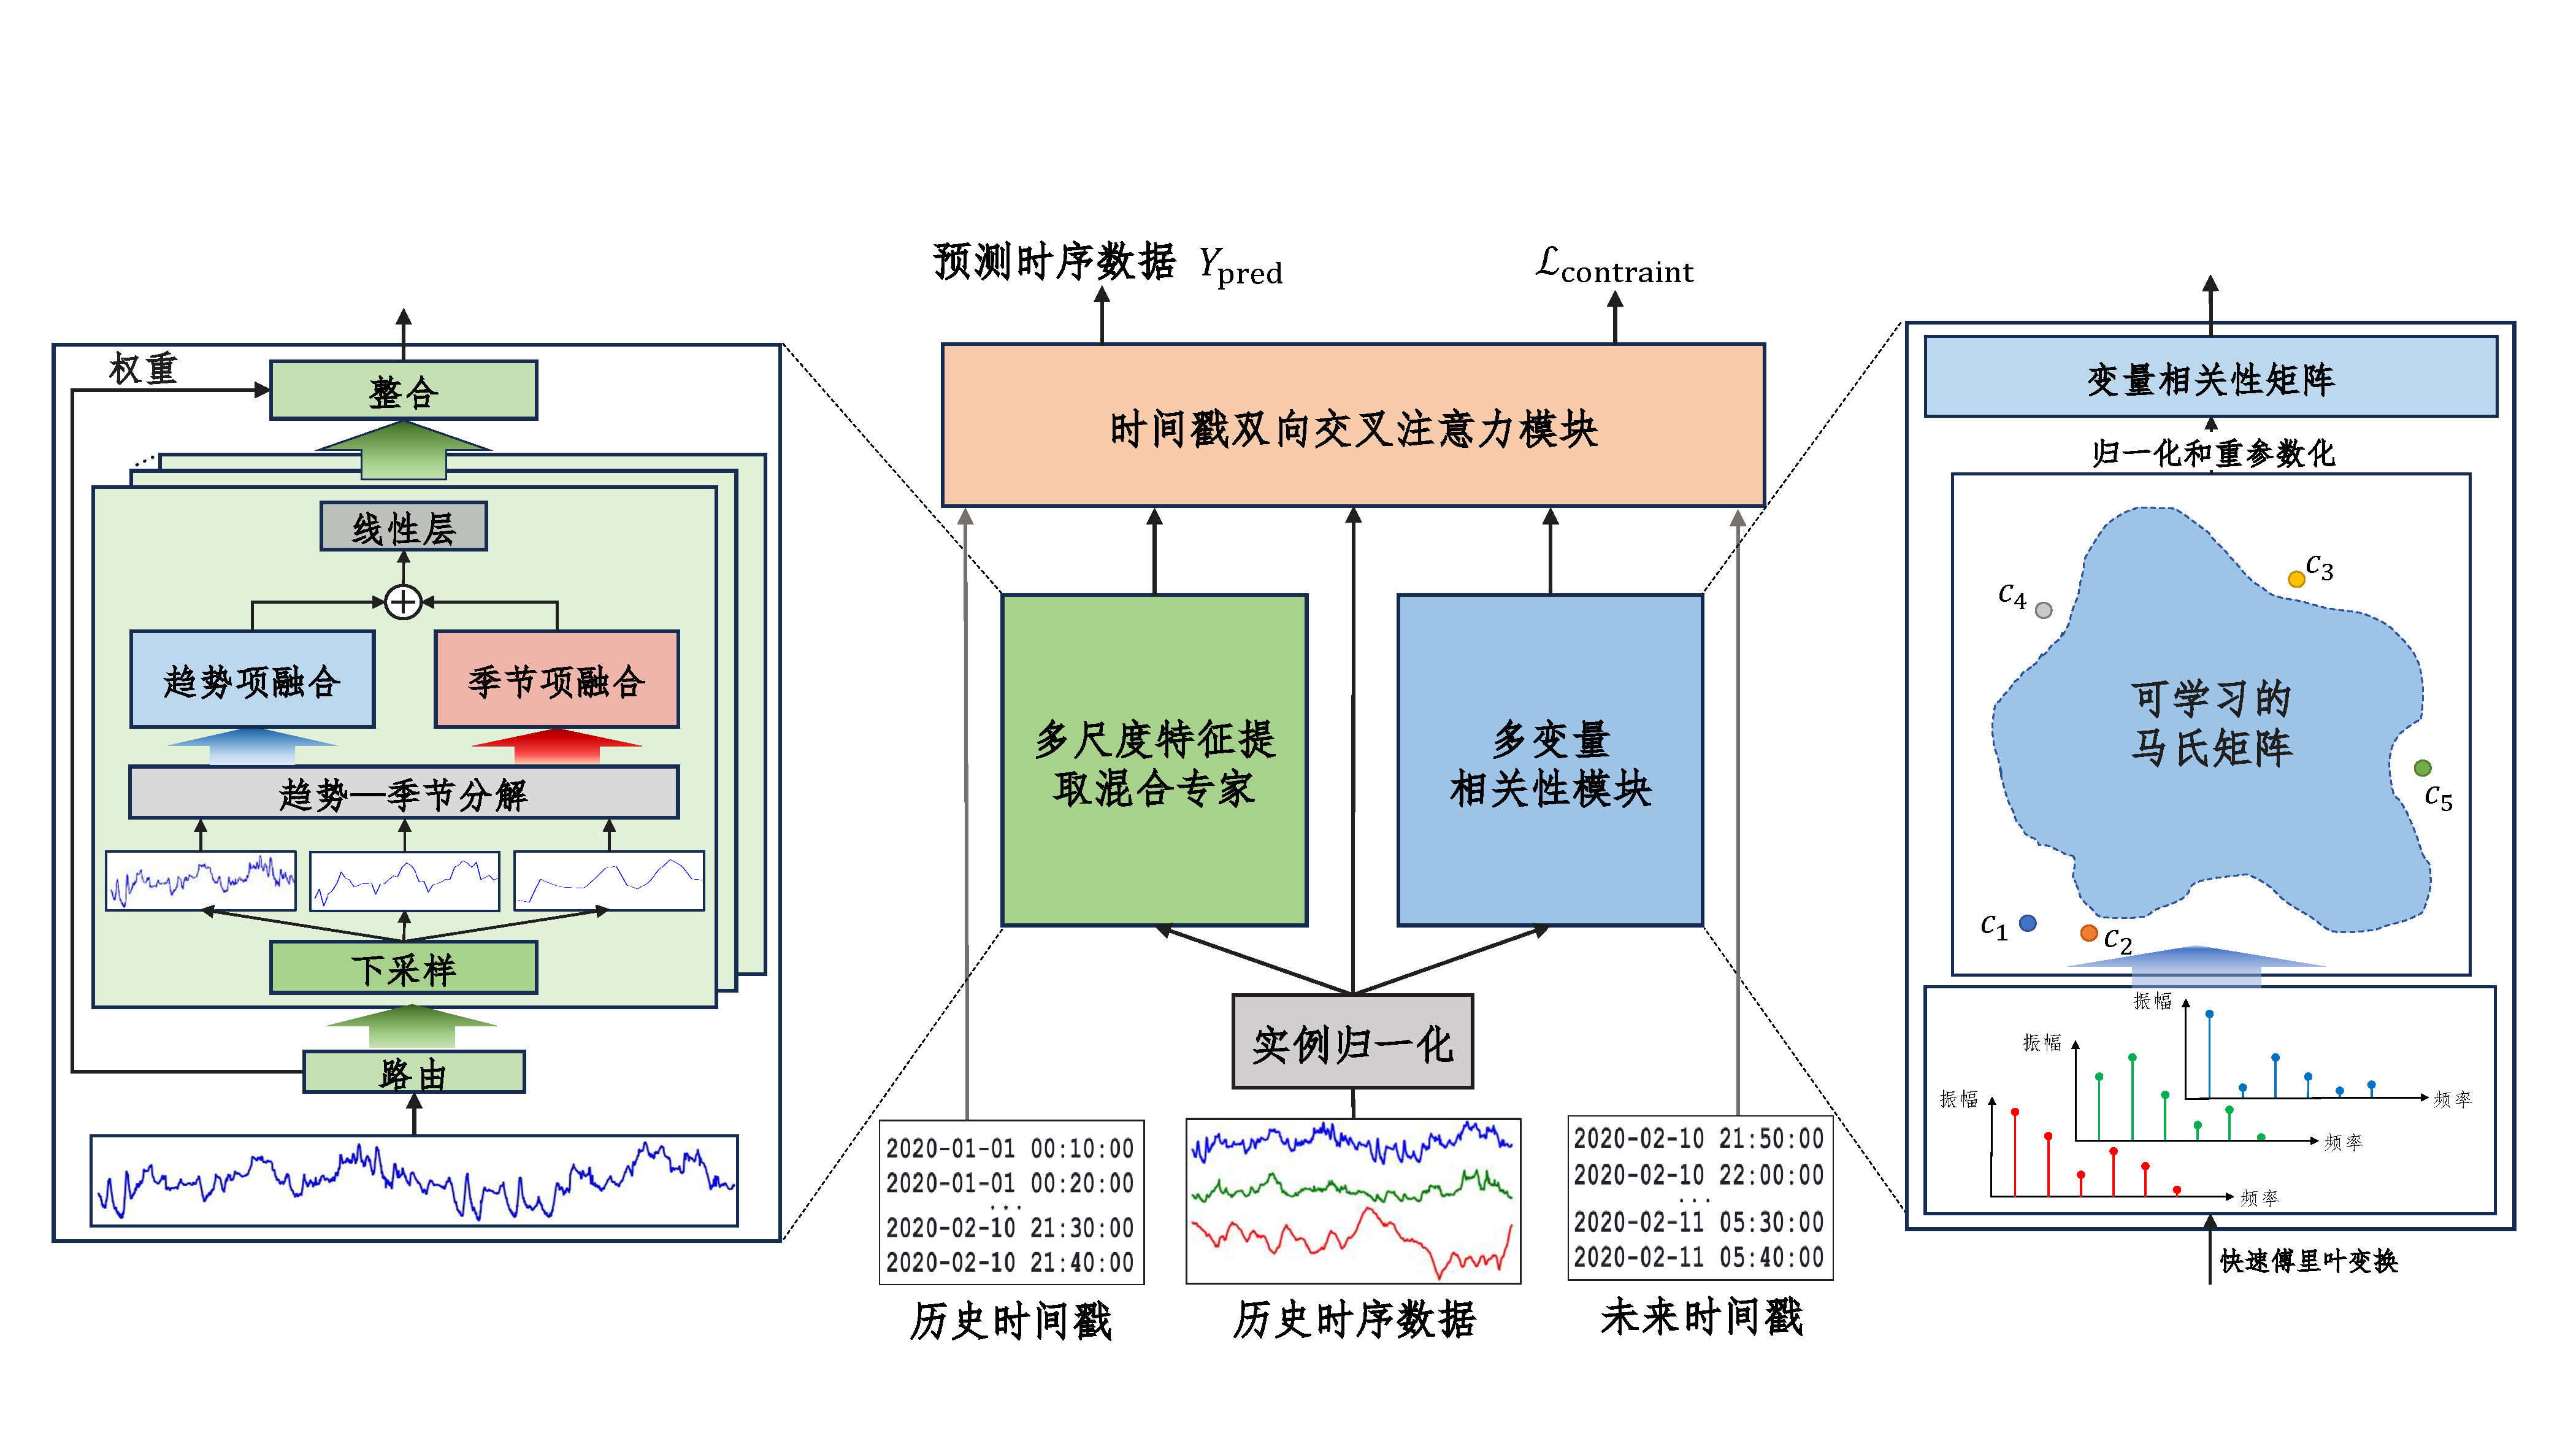
\includegraphics[width=\linewidth]{figure/bim3-pipeline.pdf}
\caption{多尺度时序混合专家与双向时间戳依赖建模的多元时序预测框架图}
\label{fig:ch3_framework}
\end{figure}


\subsection{多尺度特征提取混合专家模块}
\label{sec:ch3_msmoe}

为有效建模多元时间序列中异质的数据分布，本章提出多尺度特征提取混合专家模块。为保证计算效率，该模块以稀疏门控混合专家层~\cite{moe} 为基本结构。路由网络根据数据分布将时间序列分配给不同专家，而每个多尺度特征提取专家进一步从被路由的序列中提取多尺度时序特征。路由和特征提取均以通道独立方式进行，使模型能够保留不同变量特有的时序模式，而不是对所有通道使用同一组共享参数。

\noindent\textbf{时间序列路由\ \ } 对第 $n$ 个变量的历史序列 $X_n={X}_{:,n}\in\mathbb{R}^{T}$，首先通过两个全连接分支将其投影到低维空间，以得到用于路由的分布特征~\cite{vae}：
\begin{equation}
    {g}_n=\max\!\left(0,X_n{W}_{g}^0\right){W}_{g}^1,
\end{equation}
\begin{equation}
    {n}_n=\max\!\left(0,X_n{W}_{n}^0\right){W}_{n}^1,
\end{equation}
其中 ${W}_{g}^0,{W}_{n}^0\in\mathbb{R}^{T\times d_0}$，${W}_{g}^1,{W}_{n}^1\in\mathbb{R}^{d_0\times N_e}$，$d_0$ 为隐层维度，$N_e$ 为专家数。该路由编码以固定回看窗口长度 $T$ 为前提，训练和推理时使用相同的窗口长度。

随后采用噪声门控技术~\cite{moe} 选择概率最高的 $k$ 个专家，$k\leq N_e$，并计算相应权重：
\begin{equation}
{G}(X_n)=\mathrm{Softmax}\!\left(\mathrm{KeepTopK}\!\left({H}(X_n),k\right)\right),
\end{equation}
\begin{equation}
{H}(X_n)={W}_h\left({g}_n+\gamma\cdot\mathrm{Softplus}\!\left({n}_n\right)\right),
\end{equation}
\begin{equation}
\mathrm{KeepTopK}({v},k)_i=
\left\{
\begin{array}{ll}
v_i, & v_i \ \mbox{为}\ {v} \ \mbox{的前}\ k\ \mbox{个最大元素},\\
-\infty, & \mbox{否则}.
\end{array}
\right.
\end{equation}
其中 ${H}(X_n)\in\mathbb{R}^{N_e}$，${W}_h\in\mathbb{R}^{N_e\times N_e}$，${G}(X_n)\in\mathbb{R}^{k}$，$\gamma\sim\mathcal{N}(0,1)$。引入噪声 $\gamma$ 有利于重采样并稳定噪声门控的训练过程；Softplus 用于保持门控信号为正。${H}(X_n)$ 表示所有潜在分布的得分，${G}(X_n)$ 表示被选中专家的归一化路由权重。每个变量 $X_n$ 将根据其可能的分布被路由到 $k$ 个专家。

\noindent\textbf{多尺度特征提取专家\ \ } 路由完成后，$X_n$ 被送入 $k$ 个选中的多尺度专家。对第 $i$ 个尺度，使用平均池化得到多尺度时间序列 $\{X_n^{(0)},\ldots,X_n^{M}\}$：
\begin{equation}
X_n^{i}=\mathrm{AvgPool}_s\!\left(X_n\right),
\qquad i=0,1,\ldots,M,
\end{equation}
其中 $X_n^{(0)}=X_n$，保留最细粒度的时间变化；$X_n^{M}$ 表示最粗粒度的宏观信息。由于季节项和趋势项在时间序列分析中具有不同性质~\cite{autoformer,1990STL}，对每个尺度进行趋势—季节分解并得到所有尺度的季节项以及对应的趋势项：
\begin{equation}
{s}_n^{i},{t}_n^{i}=\mathrm{SeriesDecomp}\!\left(X_n^{i}\right),
\qquad i=0,\ldots,M,
\end{equation}
其中 ${s}_n^{i}$ 为季节项，${t}_n^{i}$ 为趋势项。

本章使用带 GELU~\cite{gelu} 激活的前馈网络分别融合季节项和趋势项，使不同尺度之间能够进行信息交互。考虑到季节项在较低尺度上具有更明显特征，而趋势项在较高尺度上更突出，本章参考 TimeMixer~\cite{timemixer} 的做法，对季节项采用自底向上的融合策略，对趋势项采用自顶向下的融合策略：
\begin{equation}
{s}_n^{i}\leftarrow {s}_n^{i}+\mathrm{FFN}_{{seas}}^{i}\!\left({s}_n^{(i-1)}\right),
\qquad i=1,\ldots,M,
\end{equation}
\begin{equation}
{t}_n^{i}\leftarrow {t}_n^{i}+\mathrm{FFN}_{{trend}}^{i}\!\left({t}_n^{(i+1)}\right),
\qquad i=M-1,\ldots,0.
\end{equation}
随后将同一尺度上的融合季节项与趋势项相加，并投影到相同隐空间用来混合特征信息。第 $e$ 个专家生成的时序特征为：
\begin{equation}
{h}_n^{(e)}=\sum_{i=0}^{M}{W}_{{mix}}^{i}\left({s}_n^{i}+{t}_n^{i}\right),
\end{equation}
其中 ${W}_{{mix}}^{i}$ 为第 $i$ 个尺度的可学习投影矩阵。

\noindent\textbf{特征聚合\ \ } 完成 $k$ 个专家的特征提取后，根据路由权重对专家输出进行加权聚合：
\begin{equation}
{z}_n=\sum_{j=1}^{k}G_j\!\left(X_n\right){h}_n^{(e_j)},
\end{equation}
其中 $e_j$ 为第 $j$ 个被选中专家的编号，$G_j(X_n)$ 为对应权重。所有变量的输出被拼接为多尺度时序特征 $X_{feat}\in\mathbb{R}^{N\times d}$。

\subsection{频域变量相关建模}
\label{sec:ch3_mcm}

变量之间的相关关系对多元时间序列预测具有重要作用。受到 DUET~\cite{duet} 的启发，本章使用可学习马氏矩阵在频域中捕捉变量相关关系，以降低不相关变量的不利影响。多元时间序列通常存在分布漂移~\cite{revin,adarnn}，而将序列变换到频域有助于缓解该问题~\cite{filternet,frets}。首先对第 $n$ 个变量计算实数快速傅里叶变换~\cite{rfft} 的幅值：
\begin{equation}
{a}_n=\left|\mathrm{rFFT}\!\left(X_n\right)\right|.
\end{equation}
其中 ${a}_n\in\mathbb{R}^{T/2}$ 表示变量 $n$ 在 $T/2$ 维频域空间中的坐标。然后利用可学习马氏矩阵~\cite{hinton_2004_maha} 度量任意两个变量在频域中的距离：
\begin{equation}
D_{i,j}=\left({a}_i-{a}_j\right)^{\top}{A}^{\top}{A}\left({a}_i-{a}_j\right),
\end{equation}
其中 ${A}$ 为可学习参数矩阵；由于对任意向量 $v$ 都有 $v^{\top}A^{\top}A v=\left\|Av\right\|_{2}^{2}\geq 0$，该构造保证 ${A}^{\top}{A}$ 半正定。实现时直接以 $\left\|{A}\left({a}_i-{a}_j\right)\right\|_{2}^{2}$ 计算。该过程以较一般且轻量的方式自适应地度量变量相关性。距离越小，表示两个变量的频域模式越接近。进一步将距离矩阵归一化到 $[0,1]$，得到变量相关性概率矩阵 ${P}\in\mathbb{R}^{N\times N}$：
\begin{equation}
P_{i,j}=
\left\{
\begin{array}{ll}
\frac{\epsilon k_{i,j}}{\max_j k_{i,j}}, & i\neq j,\\
1, & i=j,
\end{array}
\right.
\qquad
k_{i,j}=\frac{1}{D_{i,j}+\delta},
\end{equation}
其中 $k_{i,j}=1/(D_{i,j}+\delta)$ 表示两个变量的相关程度，$\delta>0$ 为稳定项，用于避免 $D_{i,j}=0$ 时出现除零，实现中取 $\delta=10^{-10}$；$\epsilon\in(0,1)$ 为缩放系数，用于避免不同变量之间绝对相关性的影响；$P_{i,j}$ 表示变量 $j$ 对变量 $i$ 有用的概率。

\noindent\textbf{重参数化\ \ } 为保留相关变量的作用并减少不相关变量的影响，本章在概率矩阵 ${P}$ 上执行伯努利重采样，得到布尔相关性掩码 $\mathcal{M}_{{cor}}\in\{0,1\}^{N\times N}$。为保证梯度能够传播，使用 Gumbel-Softmax 重参数化技术~\cite{jang2017categorical} 对离散采样过程进行可微松弛，从而在训练过程中端到端地学习变量间的稀疏相关结构。

\begin{figure}[ht!]
    \centering
    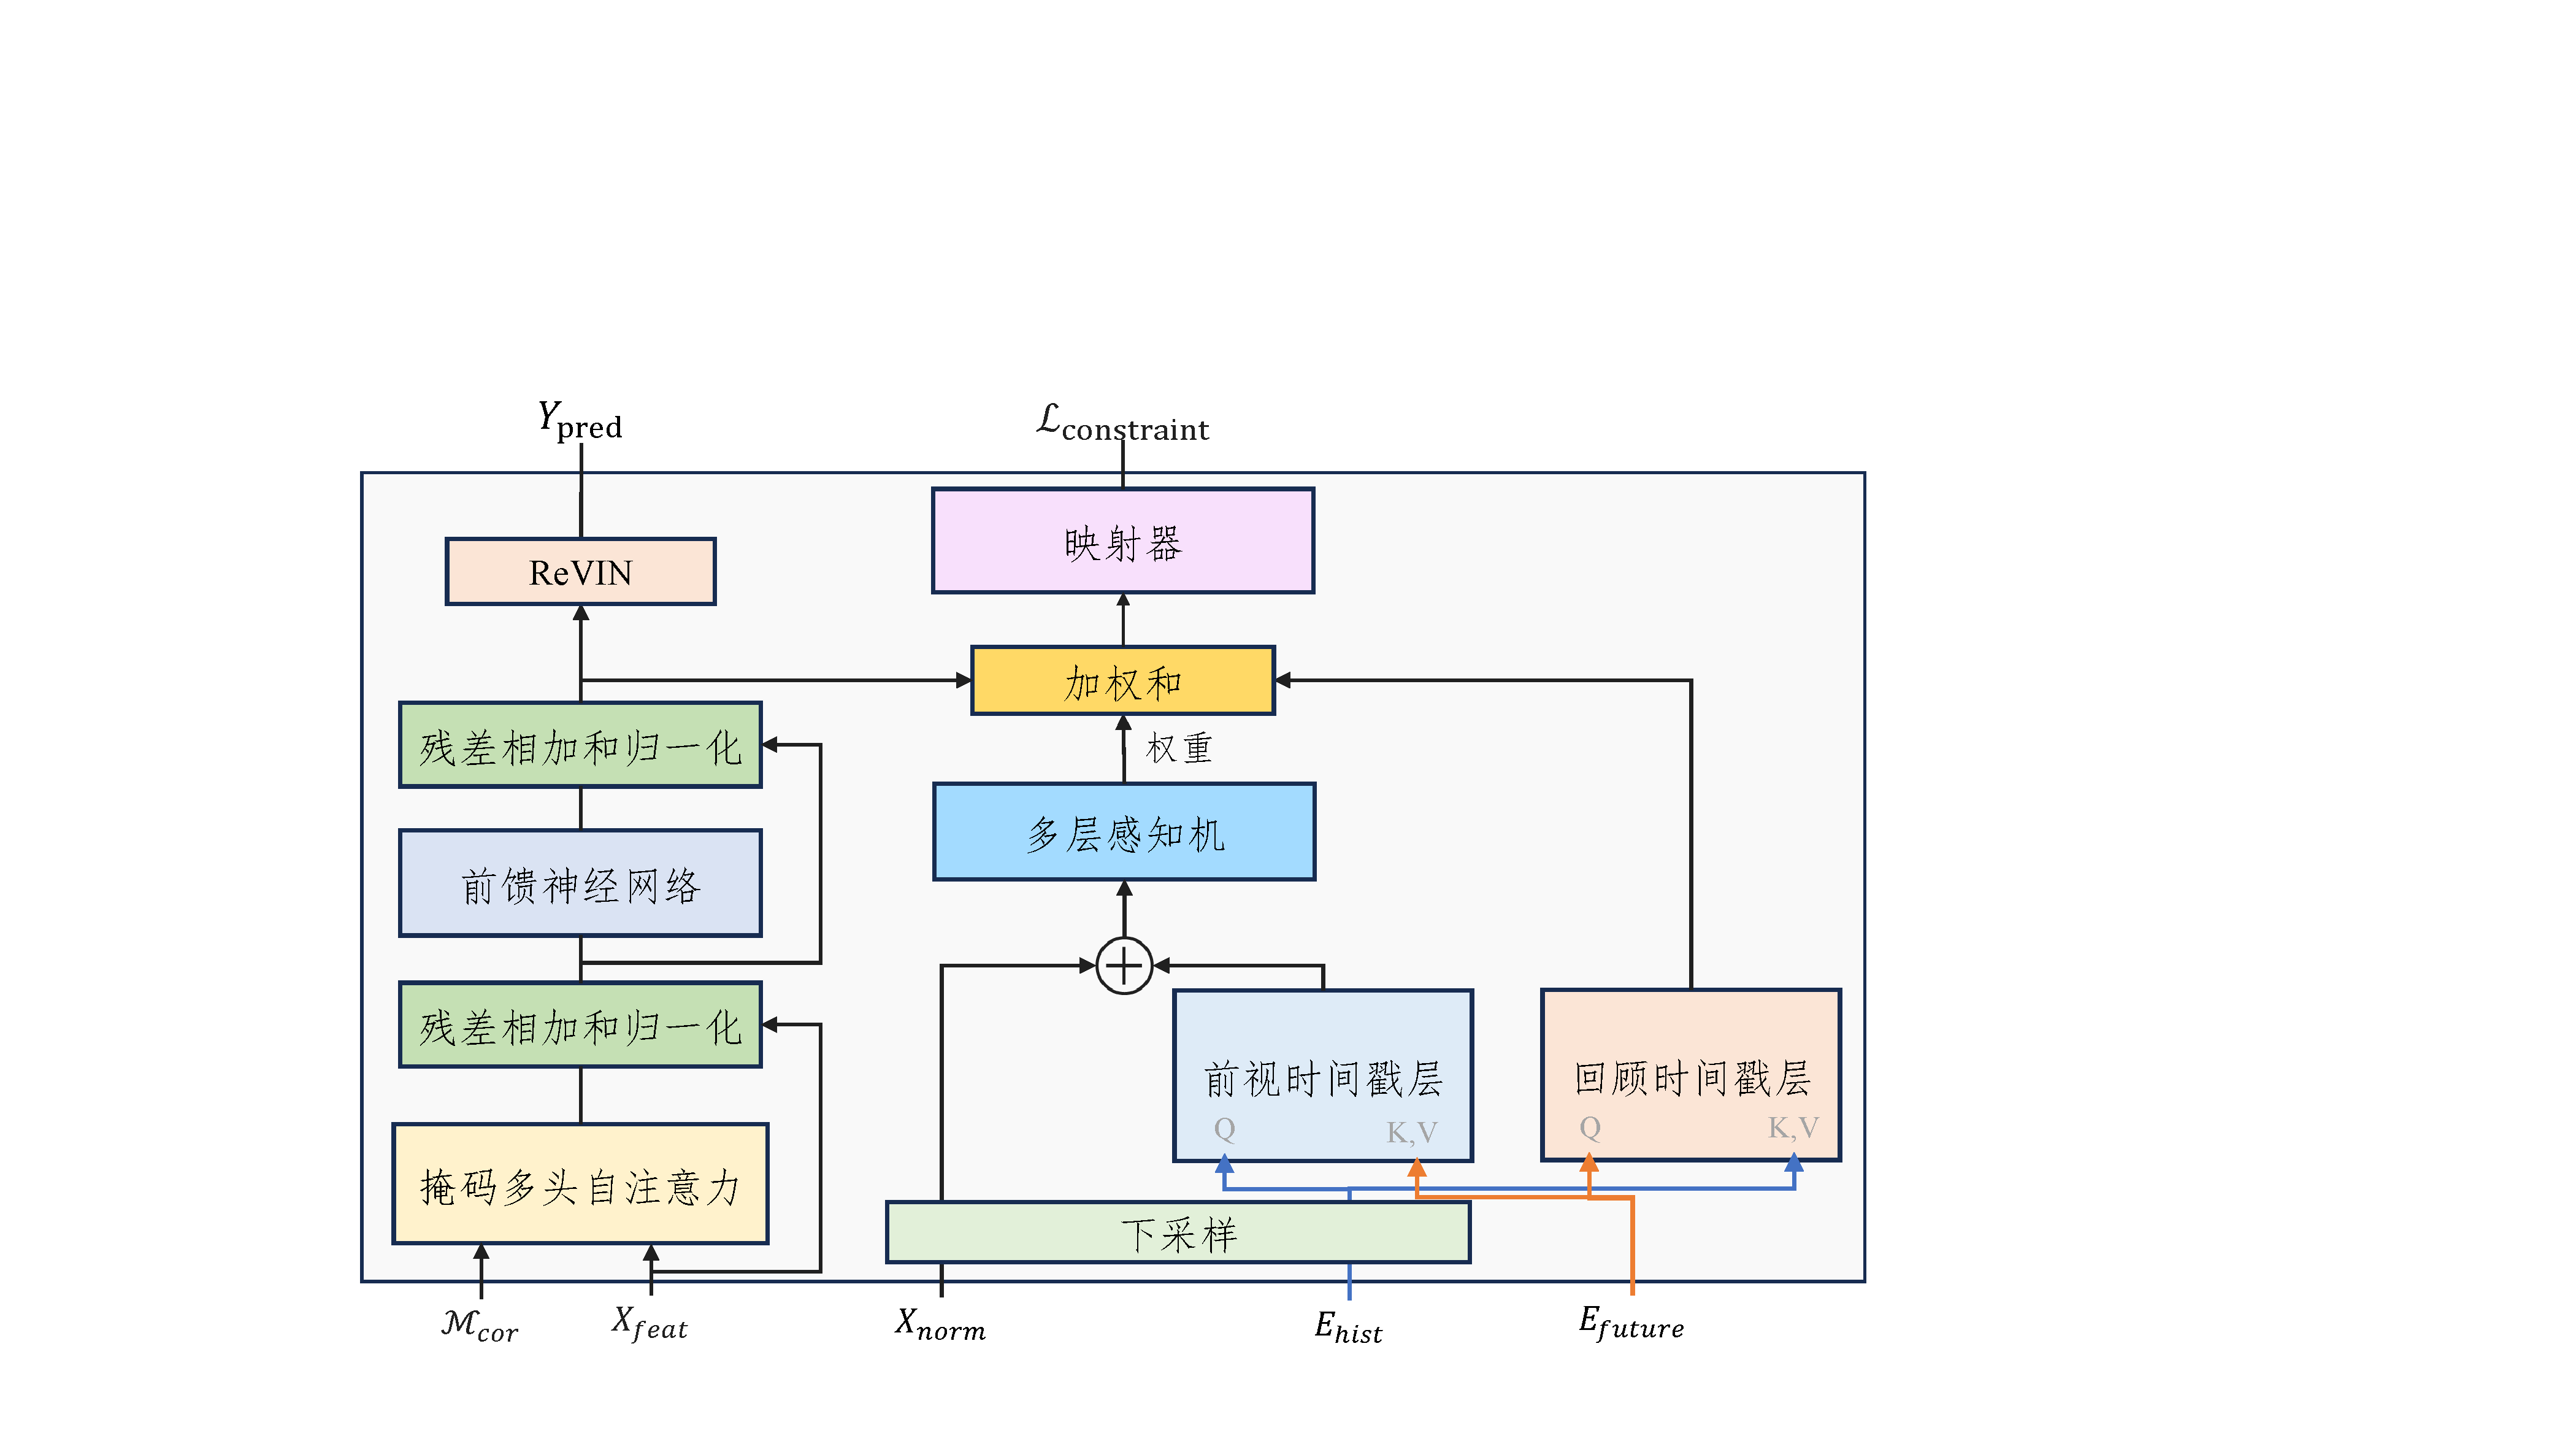
\includegraphics[width=0.95\linewidth]{figure/bim3-tdcam.pdf}
    \caption{时间戳双向交叉注意力模块结构图}
    \label{fig:ch3_tdcam}
    \end{figure}
    
\subsection{时间戳双向交叉注意力模块}
\label{sec:ch3_tdcam}

时间戳双向交叉注意力模块用于显式捕捉历史区间与未来区间之间的双向依赖，并在训练过程中引入时间戳约束。该模块首先从多尺度视角探索历史与未来的双向时间依赖，随后融合多尺度时序特征 $X_{feat}$、相关性掩码 $\mathcal{M}_{{cor}}$、归一化时间序列和时间戳信息，生成最终预测并加入辅助损失。模块结构见图~\ref{fig:ch3_tdcam}。

\noindent\textbf{双向依赖建模\ \ } 时间戳中的不同分量具有不同时间含义，因此本章分别对线性分量和周期分量进行编码。对年份 $y$，使用归一化线性编码：
\begin{equation}
e_{\mathrm{year}}=\frac{y-y_{\min}}{y_{\max}-y_{\min}},
\end{equation}
其中 $y_{\min}$ 和 $y_{\max}$ 分别为数据集中年份的最小值和最大值。对周期为 $P$ 的周期项 $v$，使用正弦和余弦编码：
\begin{equation}
e_{v}=\mathrm{concat}\left[\sin\!\left(\frac{2\pi v}{P}\right), \cos\!\left(\frac{2\pi v}{P}\right)\right].
\end{equation}
周期项包括月份、年内日、小时、分钟和星期进行编码，周期分别为 $12$、$366$、$24$、$60$ 和 $7$。历史时间戳和未来时间戳分别编码为 ${E}^{hist}$ 和 ${E}^{future}$。得到线性项和周期项的编码后，按照“年、月、日、时、分、星期”的顺序进行拼接，作为每个时间戳的最终编码。

为捕捉历史与未来时间戳之间的双向依赖，模块包含两个对称的交叉注意力分支，即前视层和回顾层。对第 $i$ 个尺度，前视层以历史时间戳嵌入作为查询、未来时间戳嵌入作为键和值，输出未来上下文特征；回顾层以未来时间戳嵌入作为查询、历史时间戳嵌入作为键和值，输出历史上下文特征。通过这种双向交叉注意力，时间依赖先通过时间戳交互被捕获，再被融入时间序列数据中，为预测提供额外上下文。

\noindent\textbf{时序特征融合\ \ } 在得到多尺度时序特征 $X_{feat}$ 和相关性掩码 $\mathcal{M}_{{cor}}$ 后，本章使用掩码注意力解码器融合时序特征。解码器以 $X_{feat}$ 作为输入序列，以 $\mathcal{M}_{{cor}}$ 作为注意力掩码，得到融合特征 $X_{fused}$。随后通过线性投影将其对齐到未来区间：
\begin{equation}
\hat{X}_{data}=X_{fused}{W}_p,
\end{equation}
其中 ${W}_p$ 将特征维度映射为预测长度 $H$。

\noindent\textbf{时间戳约束融合\ \ } 在获得前视层时间戳特征 $\bar{\mathcal{X}}_f=\{\bar{X}_f^{i}\mid i=0,\ldots,M\}$ 和回顾层时间戳特征 $\hat{\mathcal{X}}_r=\{\hat{X}_r^{i}\mid i=0,\ldots,M\}$ 后，本章对归一化历史数据 $X_{norm}$ 进行下采样，得到与各尺度对应的多尺度历史序列。对每个尺度 $i$，将前视层时间戳特征 $\bar{X}_f^{i}$ 嵌入到归一化历史序列 $X_{norm}^{i}$ 中，并使用轻量 MLP 融合前视时间戳特征与时间序列数据。该过程不仅将未来上下文注入历史序列，还在数据上引入时间戳感知约束。约束以权重形式保留，用于表示时间序列数据与时间戳特征之间的相对重要程度，从而动态调整二者对预测的贡献。进一步地，将历史区间得到的约束传播到未来区间，通过对数据项预测 $\hat{X}_{data}$ 和回顾层特征 $\hat{X}_r^{i}$ 进行加权融合实现：
\begin{equation}
{w}^{i}=\mathrm{MLP}\!\left(\bar{X}_f^{i}\oplus{X}_{norm}^{i}\right),
\end{equation}
\begin{equation}
\hat{Y}^{i}={w}^{i}\odot\left(\hat{X}_{data}\oplus\hat{X}_r^{i}\right),
\end{equation}
其中 $\bar{X}_f^{i}$ 为前视层特征，$\hat{X}_r^{i}$ 为回顾层特征，${w}^{i}\in\mathbb{R}^{N\times 2}$ 为约束权重，$\hat{Y}^{i}\in\mathbb{R}^{H\times N}$ 编码时间序列与时间戳之间的加权关系，$\oplus$ 表示拼接，$\odot$ 表示逐元素乘法。将各尺度上的 $\hat{Y}^{i}$ 收集为多尺度时间戳特征，记作 $\hat{X}_{stamp}=\hat{Y}_{ms}=\left\{\hat{Y}^{i}\mid i=0,\ldots,M\right\}$，其中每个 $\hat{Y}^{i}$ 表示第 $i$ 个尺度上时间序列数据与时间戳特征加权融合后的预测表示。

\noindent\textbf{预测输出与辅助损失\ \ } 在所有尺度上重复上述过程后，得到数据项预测 $\hat{X}_{data}$ 和多尺度时间戳特征 $\hat{X}_{stamp}$。对数据项进行逆实例归一化，得到最终预测：
\begin{equation}
Y_\mathrm{pred}=\mathrm{DeNorm}\!\left(\hat{X}_{data}\right).
\end{equation}
主损失采用 L1 损失，其中$Y_{gt}$表示真值：
\begin{equation}
\mathcal{L}_{\mathrm{main}}=\mathrm{L1Loss}\!\left(Y_\mathrm{pred},Y_\mathrm{gt}\right).
\end{equation}

为了充分整合时间戳与时间序列在不同尺度上的相关关系，本章对多尺度时间戳特征 $\hat{Y}_{ms}$ 取平均，得到 $\hat{Y}_{cons}\in\mathbb{R}^{H\times N}$：
\begin{equation}
\hat{Y}_{cons}=\mathrm{mean}\!\left(\hat{Y}_{ms}\right).
\end{equation}
随后定义了一个轻量的映射器 Mapper，该 Mapper 由带 ReLU 激活的 MLP 构成，将 $\hat{Y}_{cons}$ 投影到隐空间，得到隐向量 $V_{cons}\in\mathbb{R}^{N\times 1}$：
\begin{equation}
V_{cons}=\mathrm{Mapper}\!\left(\hat{Y}_{cons}\right).
\end{equation}
该隐向量刻画了时间戳编码与时间序列数据编码之间的特征距离。通过最小化这一特征距离，可以增强时间戳与时间序列之间的隐式相关性。时间戳约束损失定义为：
\begin{equation}
\mathcal{L}_{\mathrm{constraint}}=\epsilon_c\,\mathrm{mean}\!\left(\left|V_{cons}\right|\right),
\end{equation}
其中 $\epsilon_c$ 为人工调节的约束强度系数。该损失鼓励模型将时间戳特征和先验上下文纳入预测过程，从而在训练中施加时间戳感知约束。为平衡专家负载，另加入重要性损失 $\mathcal{L}_{\mathrm{importance}}$~\cite{moe}。最终总损失函数为：
\begin{equation}
\mathcal{L}=\mathcal{L}_{\mathrm{main}}+\mathcal{L}_{\mathrm{constraint}}+\mathcal{L}_{\mathrm{importance}}.
\end{equation}

\section{实验结果与分析}

\begin{table}[t!]
    \caption{多元时间序列数据集统计信息}
    \label{tab:ch3-datasets}
    % \footnotesize
    \resizebox{\linewidth}{!}{
    \begin{tabular}{ccccccc}
    \toprule
        \textbf{数据集} & \textbf{领域} & \textbf{采样频率} & \textbf{样本数} & \textbf{变量数} & \textbf{划分}  & \textbf{描述}\\ 
    \midrule
        Electricity  & 电力 & 1小时    & 26,304      & 321      & 7:1:2 & 记录 2012 年至 2014 年每小时电力消耗，单位为 kWh\\
        ETTh1        & 电力 & 1小时     & 14,400      & 7        & 6:2:2 & 电力变压器 1，包含油温、有用负荷等 7 项指标\\
        ETTh2        & 电力 & 1小时    & 14,400      & 7        & 6:2:2 & 电力变压器 2，包含油温、有用负荷等 7 项指标\\
        ETTm1        & 电力 & 15分钟   & 57,600      & 7        & 6:2:2 & 电力变压器 1，包含油温、有用负荷等 7 项指标\\
        ETTm2        & 电力 & 15分钟   & 57,600      & 7        & 6:2:2 & 电力变压器 2，包含油温、有用负荷等 7 项指标\\
        Exchange & 经济    & 1天      & 7,588       & 8        & 7:1:2 & 收集 8 个国家的每日汇率\\
        ILI          & 医疗      & 1周     & 966        & 7        & 7:1:2 & 美国疾病控制与预防中心记录的流感样疾病患者指标\\
        Traffic      & 交通     & 1小时    & 17,544      & 862      & 7:1:2 & 旧金山湾区高速公路 862 个传感器测得的道路占用率\\
        Solar        & 能源      & 10分钟   & 52,560      & 137      & 6:2:2 & 阿拉巴马州 137 个光伏电站的太阳能发电记录 \\
        Weather      & 环境 & 10分钟   & 52,696      & 21       & 7:1:2 & 2020 年全年记录，包含 21 项气象指标\\
    \bottomrule
    \end{tabular}
    }
\end{table}

\subsection{数据集介绍}

实验使用 10 个公开真实数据集~\cite{tfb}，包括 Electricity、ETTh1、ETTh2、ETTm1、ETTm2、Exchange、ILI、Solar、Traffic 和 Weather。这些数据集覆盖电力、金融、医疗、交通、能源和环境等领域，各数据集的统计信息如表~\ref{tab:ch3-datasets} 所示。实验采用滑动窗口方式构造训练、验证和测试样本：从完整序列中连续截取长度为历史窗口加预测窗口的片段，前段作为模型输入，后段作为监督目标。输入数据使用 z-score 归一化按变量进行归一化处理，测试时对预测结果进行逆归一化后再计算指标。为了公平比较，实验不采用 Drop Last 技巧~\cite{foundts}，并保留与基准方法一致的数据划分。

\subsection{对比方法}

为全面评估不同技术路线的方法在预测精度上的表现，本章节选择三类具有代表性的近期基线方法进行对比。第一类为线性与轻量模型，包括 DLinear~\cite{dlinear}、FITS~\cite{fits} 和 TimeLinear~\cite{timester}，其特点是结构简单、计算开销较低，常作为时序预测的强基线。第二类为 Transformer 类模型，包括 PatchTST~\cite{patchtst}、iTransformer~\cite{itransformer}、Crossformer~\cite{crossformer}、SOFTS~\cite{softs} 和 DUET~\cite{duet}，这些方法分别通过时间块、变量令牌、跨维注意力、序列核和聚类等方式改进时序 Transformer。第三类为多尺度与频域模型，包括 TimeMixer~\cite{timemixer}、Pathformer~\cite{pathformer}、PDF~\cite{pdf} 和 TimesNet~\cite{timesnet}，它们从多尺度分解、自适应分块、周期解耦和二维时序变换等角度增强多尺度时序建模能力。

为保证公平比较，本章选择各方法在候选回看窗口下的最佳结果，并重新运行所有基线的官方代码得到实验结果。

评价指标为均方误差（Mean Square Error，MSE）和平均绝对误差（Mean Absolute Error，MAE）。为便于描述，记测试集中共有$K$对多元时间序列数据$(Y_{\mathrm{pred}}, Y_{\mathrm{gt}})$（分别表示真实数据与预测结果），每条数据包含$N$个时间变量在$H$个时间步的数值。则各指标定义如下：
\begin{equation}
    \mathrm{MSE}(Y_{\mathrm{pred}}, Y_{\mathrm{gt}}) = \frac{1}{KHN}\sum_{h=1}^{H}\sum_{n=1}^{N}
    \left(Y_{\mathrm{pred}}[h,n] - Y_{\mathrm{gt}}[h,n]\right)^{2}
\end{equation}
\begin{equation}
    \mathrm{MAE}(Y_{\mathrm{pred}}, Y_{\mathrm{gt}}) = \frac{1}{KHN}\sum_{h=1}^{H}\sum_{n=1}^{N}
    \left|Y_{\mathrm{pred}}[h,n] - Y_{\mathrm{gt}}[h,n]\right|
\end{equation}

\subsection{实现细节}

实验基于 PyTorch~\cite{pytorch} 实现，使用 ADAM 优化器~\cite{adam}，初始学习率设为 $0.02$。学习率采用分段衰减策略，即在训练初期保持初始学习率，随后按比例逐步降低。训练轮数设置为 $100$，并采用早停机制，当验证集指标连续 $10$ 轮未改善时停止训练，保存验证集上最优的模型权重。由于各数据集的序列长度和样本规模差异较大，批量大小根据数据集在 $8$ 到 $256$ 之间调整，以在避免显存溢出的同时提高 GPU 利用率。输入数据在训练、验证和测试阶段均使用训练集统计量进行归一化。推理时对预测结果进行逆归一化，并使用与验证集相同的数据窗口设置和指标计算方式。实验在单张 NVIDIA A100 80GB GPU 上完成。
预测长度方面，ILI 数据集使用 $H\in\{24,36,48,60\}$，其余数据集使用 $H\in\{96,192,336,720\}$。回看窗口方面，ILI 数据集使用 $T\in\{96,104\}$，其余数据集使用 $T\in\{96,336,720\}$；为保证公平比较，每个基线报告其在所选回看窗口下的最佳结果。

\begin{table}[ht!]
    \centering
    \caption{多元时间序列预测方法主实验结果}
    
    \label{tab:ch3-main-res}
    
    \resizebox{\linewidth}{!}{
        \begin{tabular}{cc|cc|cc|cc|cc|cc|cc|cc|cc|cc|cc|cc|cc|cc}
        \toprule
            \multicolumn{2}{c|}{方法} & \multicolumn{2}{c|}{本章方法} & \multicolumn{2}{c|}{DUET} & \multicolumn{2}{c|}{TimeLinear} & \multicolumn{2}{c|}{PDF} & \multicolumn{2}{c|}{FITS} & \multicolumn{2}{c|}{Pathformer} & \multicolumn{2}{c|}{TimeMixer} & \multicolumn{2}{c|}{iTransformer} & \multicolumn{2}{c|}{SOFTS} & \multicolumn{2}{c|}{PatchTST} & \multicolumn{2}{c|}{Crossformer} & \multicolumn{2}{c|}{TimesNet} & \multicolumn{2}{c}{DLinear} \\
            \midrule
            \multicolumn{2}{c|}{指标} & MSE & MAE & MSE & MAE & MSE & MAE & MSE & MAE & MSE & MAE & MSE & MAE & MSE & MAE & MSE & MAE & MSE & MAE & MSE & MAE & MSE & MAE & MSE & MAE & MSE & MAE \\
        \midrule    %% ECL
            \multirow{4}{*}{\rotatebox[origin=c]{90}{Electricity}} & 96 & \textcolor{red}{\textbf{0.126}} & \textcolor{red}{\textbf{0.217}} & 0.128&0.219 & 0.140&0.234 & \textcolor{blue}{\underline{0.127}}&0.221 & 0.153&0.259 & 0.134&0.222 & 0.129&0.225 & 0.152&0.248 & 0.145&0.235 & 0.143&0.247 & 0.132&\textcolor{blue}{\underline{0.218}} & 0.168&0.271 & 0.140&0.237 \\
            
            & 192 & \textcolor{red}{\textbf{0.145}}&\textcolor{red}{\textbf{0.235}} & \textcolor{blue}{\underline{0.145}}&0.237 & 0.155&0.247 & 0.147&0.240 & 0.167&0.271 & 0.155&0.252 & 0.151&0.245 & 0.152&0.248 & 0.162&0.252 & 0.149&0.244 & 0.181&\textcolor{blue}{\underline{0.236}} & 0.185&0.287 &0.153&0.250 \\
            
            & 336 & \textcolor{red}{\textbf{0.162}}&\textcolor{red}{\textbf{0.253}} & 0.163&\textcolor{blue}{\underline{0.254}} & 0.169&0.265 & \textcolor{blue}{\underline{0.163}}&0.256 & 0.182&0.285 & 0.172&0.268 & 0.167&0.256 & 0.168&0.264 & 0.182&0.273 &0.168&0.260 & 0.167&0.263 & 0.204&0.305 & 0.169&0.268 \\
            
            & 720 & \textcolor{red}{\textbf{0.190}}&\textcolor{red}{\textbf{0.278}} & \textcolor{blue}{\underline{0.193}}&\textcolor{blue}{\underline{0.280}} & 0.198&0.291 & 0.196&0.287 & 0.220&0.315 & 0.211&0.302 & 0.196&0.289 & 0.194&0.287 & 0.215&0.303 & 0.198&0.290 & 0.225&0.312 & 0.223&0.322 & 0.204&0.300 \\
        \midrule    %% ETTh1
            \multirow{4}{*}{\rotatebox[origin=c]{90}{ETTh1}} & 96 & \textcolor{red}{\textbf{0.354}}&\textcolor{red}{\textbf{0.386}} & \textcolor{blue}{\underline{0.354}}&\textcolor{blue}{\underline{0.387}} & 0.377&0.391 & 0.361&0.392 & 0.372&0.396 & 0.383&0.390 & 0.361&0.390 & 0.400&0.425 & 0.382&0.401 & 0.370&0.400 & 0.409&0.434 & 0.389&0.412 & 0.384&0.405 \\
            
            & 192 & \textcolor{blue}{\underline{0.399}}&\textcolor{red}{\textbf{0.412}} & 0.400&0.417 & 0.424&0.419 & \textcolor{red}{\textbf{0.391}}&0.415 & 0.405&0.416 & 0.442&0.420 & 0.409&\textcolor{blue}{\underline{0.414}} & 0.427&0.443 & 0.436&0.432 & 0.413&0.429 & 0.424&0.451 & 0.439&0.442 & 0.443&0.450 \\
            
            & 336 & \textcolor{red}{\textbf{0.419}}&\textcolor{red}{\textbf{0.429}} & 0.422&0.431 & 0.463&0.438 & \textcolor{blue}{\underline{0.419}}&0.430 & 0.423&0.439 & 0.458&\textcolor{blue}{\underline{0.430}} & 0.432&0.435 & 0.457&0.465 & 0.479&0.452 & 0.422&0.440 & 0.433&0.461 & 0.495&0.471 & 0.447&0.448 \\
            
            & 720 & \textcolor{blue}{\underline{0.431}}&0.458 & 0.432&0.458 & 0.465&\textcolor{blue}{\underline{0.456}} & 0.468&0.482 & \textcolor{red}{\textbf{0.426}}&\textcolor{red}{\textbf{0.448}} & 0.491&0.462 & 0.445&0.465 & 0.492&0.485 & 0.499&0.488 & 0.447&0.468 & 0.691&0.634 & 0.520&0.496 & 0.504&0.515 \\
        \midrule    %% ETTh2
            \multirow{4}{*}{\rotatebox[origin=c]{90}{ETTh2}} & 96 & \textcolor{red}{\textbf{0.272}}&\textcolor{red}{\textbf{0.336}} & \textcolor{blue}{\underline{0.273}}&\textcolor{blue}{\underline{0.337}} & 0.285&0.338 & 0.276&0.342 & 0.276&0.338 & 0.283&0.343 & 0.285&0.340 & 0.299&0.359 & 0.297&0.348 & 0.277&0.337 & 0.283&0.351 & 0.337&0.371 & 0.290&0.353\\
            
            & 192 & \textcolor{red}{\textbf{0.333}}&\textcolor{red}{\textbf{0.375}} & 0.335&0.377 & 0.372&0.390 & 0.334&0.375 & \textcolor{blue}{\underline{0.334}}&\textcolor{blue}{\underline{0.375}} & 0.349&0.376 & 0.375&0.391 & 0.377&0.406 & 0.374&0.394 & 0.341&0.382 & 0.356&0.384 & 0.405&0.415 & 0.388&0.422 \\
            
            & 336 & \textcolor{red}{\textbf{0.358}}&0.401 & 0.361&0.397 & 0.395&0.401 & 0.360&0.401 & 0.360&\textcolor{blue}{\underline{0.395}} & \textcolor{blue}{\underline{0.359}}&\textcolor{red}{\textbf{0.382}} & 0.387&0.411 & 0.429&0.442 & 0.419&0.431 & 0.377&0.416 & 0.359&0.410 & 0.452&0.451 & 0.463&0.472 \\
            
            & 720 & 0.384&\textcolor{blue}{\underline{0.422}} & \textcolor{blue}{\underline{0.379}}&0.423 & \textcolor{red}{\textbf{0.367}}&\textcolor{red}{\textbf{0.408}} & 0.398&0.438 & 0.380&0.423 & 0.413&0.431 & 0.413&0.432 & 0.444&0.466 & 0.427&0.445 & 0.397&0.432 & 0.399&0.457 & 0.435&0.448 & 0.733&0.606 \\
        \midrule    %% ETTm1
            \multirow{4}{*}{\rotatebox[origin=c]{90}{ETTm1}} & 96 & \textcolor{red}{\textbf{0.280}}&\textcolor{red}{\textbf{0.335}} & 0.281&\textcolor{blue}{\underline{0.336}} & 0.325&0.364 & \textcolor{blue}{\underline{0.281}}&0.338 & 0.306&0.348 & 0.317&0.345 & 0.321&0.356 & 0.311&0.366 & 0.328&0.364 & 0.290&0.344 & 0.315&0.371 & 0.334&0.375 & 0.301&0.345 \\
            
            & 192 & \textcolor{red}{\textbf{0.322}}&\textcolor{red}{\textbf{0.360}} & \textcolor{blue}{\underline{0.323}}&0.363 & 0.365&0.380 & 0.324&\textcolor{blue}{\underline{0.363}} & 0.338&0.367 & 0.366&0.369 & 0.327&0.365 & 0.348&0.385 & 0.372&0.389 & 0.333&0.371 & 0.342&0.383 & 0.409&0.414 & 0.336&0.366 \\
            
            & 336 & \textcolor{red}{\textbf{0.348}}&\textcolor{red}{\textbf{0.378}} & \textcolor{blue}{\underline{0.349}}&0.380 & 0.395&0.401 & 0.358&0.383 & 0.368&0.384 & 0.387&0.389 & 0.365&\textcolor{blue}{\underline{0.379}} & 0.379&0.405 & 0.416&0.417 & 0.369&0.392 & 0.395&0.418 & 0.414&0.422 & 0.372&0.389 \\
            
            & 720 & \textcolor{red}{\textbf{0.403}}&\textcolor{red}{\textbf{0.410}} & 0.405&\textcolor{blue}{\underline{0.412}} & 0.455&0.433 & \textcolor{blue}{\underline{0.405}}&0.414 & 0.421&0.413 & 0.460&0.432 & 0.414&0.416 & 0.443&0.444 & 0.474&0.450 & 0.416&0.420 & 0.560&0.518 & 0.510&0.472 & 0.426&0.423 \\
        \midrule    %% ETTm2
            \multirow{4}{*}{\rotatebox[origin=c]{90}{ETTm2}} & 96 & \textcolor{red}{\textbf{0.160}}&\textcolor{red}{\textbf{0.249}} & \textcolor{blue}{\underline{0.162}}&0.251 & 0.167&0.253 & 0.163&0.252 & 0.165&0.254 & 0.170&\textcolor{blue}{\underline{0.249}} & 0.167&0.253 & 0.179&0.273 & 0.182&0.262 & 0.166&0.256 & 0.172&0.261 & 0.189&0.266 & 0.172&0.267 \\
            
            & 192 & \textcolor{blue}{\underline{0.218}}&\textcolor{red}{\textbf{0.286}} & \textcolor{red}{\textbf{0.215}}&\textcolor{blue}{\underline{0.289}} & 0.233&0.291 & 0.224&0.296 & 0.222&0.291 & 0.232&0.291 & 0.224&0.296 & 0.242&0.315 & 0.246&0.305 & 0.223&0.296 & 0.222&0.298 & 0.252&0.307 & 0.237&0.314 \\
            
            & 336 & \textcolor{red}{\textbf{0.268}}&\textcolor{red}{\textbf{0.321}} & \textcolor{blue}{\underline{0.269}}&\textcolor{blue}{\underline{0.323}} & 0.294&0.331 & 0.277&0.332 & 0.273&0.326 & 0.294&0.331 & 0.279&0.331 & 0.291&0.345 & 0.319&0.352 & 0.274&0.329 & 0.283&0.332 & 0.323&0.350 & 0.294&0.359 \\
            
            & 720 & \textcolor{red}{\textbf{0.349}}&\textcolor{red}{\textbf{0.373}} & \textcolor{blue}{\underline{0.351}}&\textcolor{blue}{\underline{0.374}} & 0.395&0.390 & 0.354&0.378 & 0.359&0.381 & 0.384&0.385 & 0.360&0.381 & 0.377&0.397 & 0.411&0.405 & 0.362&0.385 & 0.353&0.381 & 0.418&0.405 & 0.426&0.439 \\
        \midrule    %% Exchange
            \multirow{4}{*}{\rotatebox[origin=c]{90}{Exchange}} & 96 & \textcolor{blue}{\underline{0.082}}&\textcolor{red}{\textbf{0.201}} & \textcolor{red}{\textbf{0.079}}&0.203 & 0.087&0.206 & 0.082&\textcolor{blue}{\underline{0.202}} & 0.087&0.208 & 0.094&0.214 & 0.085&0.203 & 0.086&0.206 & 0.088&0.206 & 0.082&0.203 & 0.088&0.210 & 0.105&0.235 & 0.085&0.209 \\
            
            & 192 & \textcolor{red}{\textbf{0.164}}&\textcolor{red}{\textbf{0.290}} & \textcolor{blue}{\underline{0.165}}&\textcolor{blue}{\underline{0.292}} & 0.180&0.301 & 0.172&0.294 & 0.179&0.303 & 0.190&0.313 & 0.180&0.302 & 0.180&0.304 & 0.187&0.309 & 0.171&0.293 & 0.174&0.302 & 0.222&0.345 & 0.165&0.296 \\
            
            & 336 & \textcolor{red}{\textbf{0.286}}&\textcolor{red}{\textbf{0.392}} & \textcolor{blue}{\underline{0.294}}&\textcolor{blue}{\underline{0.393}} & 0.341&0.420 & 0.322&0.410 & 0.325&0.413 & 0.388&0.447 & 0.363&0.438 & 0.338&0.422 & 0.337&0.421 & 0.316&0.406 & 0.331&0.420 & 0.363&0.439 & 0.333&0.441 \\
            
            & 720 & \textcolor{red}{\textbf{0.578}}&\textcolor{red}{\textbf{0.576}} & \textcolor{blue}{\underline{0.584}}&\textcolor{blue}{\underline{0.580}} & 0.805&0.641 & 0.830&0.686 & 0.846&0.695 & 0.938&0.735 & 1.036&0.755 & 0.853&0.696 & 0.849&0.698 & 0.884&0.701 & 0.873&0.752 & 0.931&0.734 & 0.898&0.725 \\
        \midrule    %% ILI
            \multirow{4}{*}{\rotatebox[origin=c]{90}{ILI}} & 24 & \textcolor{red}{\textbf{1.523}}&0.776 & \textcolor{blue}{\underline{1.577}}&\textcolor{red}{\textbf{0.760}} & 2.427&1.068 & 1.801&0.872 & 2.180&0.998 & 2.075&0.923 & 1.645&\textcolor{blue}{\underline{0.764}} & 2.333&1.036 & 1.817&0.871 & 1.679&0.882 & 1.914&0.898 & 1.813&0.888 & 2.279&1.061 \\
            
            & 36 & \textcolor{red}{\textbf{1.660}}&\textcolor{red}{\textbf{0.802}} & 1.732&0.809 & 2.224&1.034 & 1.723&0.844 & 2.236&1.022 & 1.922&0.875 & \textcolor{blue}{\underline{1.676}}&0.827 & 2.238&1.015 & 2.237&1.034 & 1.695&\textcolor{blue}{\underline{0.805}} & 2.547&1.161 & 2.679&0.986 & 2.235&1.059 \\
            
            & 48 & \textcolor{red}{\textbf{1.607}}&\textcolor{red}{\textbf{0.793}} & 1.682&0.819 & 2.026&0.950 & 1.890&0.936 & 2.278&1.067 & 1.981&0.900 & \textcolor{blue}{\underline{1.658}}&\textcolor{blue}{\underline{0.841}} & 2.215&1.028 & 2.223&1.028 & 1.783&0.864 & 2.711&1.257 & 2.584&0.938 & 2.298&1.079 \\
            
            & 60 & \textcolor{red}{\textbf{1.667}}&\textcolor{red}{\textbf{0.810}} & \textcolor{blue}{\underline{1.670}}&\textcolor{blue}{\underline{0.815}} & 2.102&1.013 & 1.822&0.949 & 2.634&1.130 & 2.001&0.930 & 1.688&0.879 & 2.086&1.014 & 2.157&1.030 & 1.831&0.892 & 2.825&1.288 & 1.981&0.894 & 2.573&1.157 \\
        \midrule    %% Solar
            \multirow{4}{*}{\rotatebox[origin=c]{90}{Solar}} & 96 & \textcolor{red}{\textbf{0.168}}&\textcolor{red}{\textbf{0.198}} & 0.173&\textcolor{blue}{\underline{0.200}} & 0.199&0.272 & 0.184&0.245 & 0.211&0.257 & 0.215&0.234 & \textcolor{blue}{\underline{0.172}}&0.220 & 0.189&0.264 & 0.201&0.232 & 0.173&0.234 & 0.187&0.229 & 0.194&0.265 & 0.222&0.291 \\
            
            & 192 & \textcolor{red}{\textbf{0.184}}&\textcolor{red}{\textbf{0.210}} & \textcolor{blue}{\underline{0.189}}&\textcolor{blue}{\underline{0.215}} & 0.219&0.288 & 0.200&0.261 & 0.224&0.269 & 0.194&0.217 & 0.190&0.249 & 0.208&0.272 & 0.229&0.254 & 0.204&0.302 & 0.202&0.248 & 0.201&0.274 & 0.250&0.310 \\
            
            & 336 & \textcolor{red}{\textbf{0.185}}&\textcolor{red}{\textbf{0.215}} & 0.199&0.221 & 0.237&0.306 & 0.209&0.365 & 0.247&0.275 & \textcolor{blue}{\underline{0.195}}&\textcolor{blue}{\underline{0.220}} & 0.201&0.254 & 0.215&0.279 & 0.242&0.268 & 0.212&0.293 & 0.218&0.294 & 0.211&0.289 & 0.269&0.323 \\
            
            & 720 & \textcolor{red}{\textbf{0.196}}&\textcolor{red}{\textbf{0.221}} & \textcolor{blue}{\underline{0.206}}&\textcolor{blue}{\underline{0.223}} & 0.256&0.294 & 0.214&0.269 & 0.253&0.276 & 0.208&0.237 & 0.215&0.250 & 0.224&0.287 & 0.244&0.271 & 0.215&0.307 & 0.226&0.301 & 0.230&0.306 & 0.271&0.327 \\
        \midrule    %% Traffic
            \multirow{4}{*}{\rotatebox[origin=c]{90}{Traffic}} & 96 & \textcolor{red}{\textbf{0.359}}&\textcolor{red}{\textbf{0.237}} & \textcolor{blue}{\underline{0.360}}&\textcolor{blue}{\underline{0.238}} & 0.459&0.293 & 0.369&0.245 & 0.407&0.289 & 0.383&0.250 & 0.366&0.251 & 0.362&0.260 & 0.376&0.251 & 0.371&0.254 & 0.485&0.266 & 0.589&0.315 & 0.413&0.287 \\
            
            & 192 & \textcolor{blue}{\underline{0.382}}&\textcolor{red}{\textbf{0.249}} & 0.384&\textcolor{blue}{\underline{0.250}} & 0.467&0.299 & \textcolor{red}{\textbf{0.377}}&0.251 & 0.418&0.292 & 0.401&0.257 & 0.389&0.261 & 0.384&0.276 & 0.397&0.261 & 0.386&0.263 & 0.501&0.278 & 0.618&0.324 & 0.424&0.290 \\
            
            & 336 & \textcolor{blue}{\underline{0.395}}&\textcolor{red}{\textbf{0.259}} & 0.396&0.261 & 0.480&0.305 & \textcolor{red}{\textbf{0.393}}&0.269 & 0.427&0.297 & 0.423&\textcolor{blue}{\underline{0.261}} & 0.412&0.272 & 0.395&0.268 & 0.415&0.269 & 0.396&0.272 & 0.518&0.280 & 0.632&0.336 & 0.438&0.298 \\
            
            & 720 & \textcolor{red}{\textbf{0.435}}&\textcolor{red}{\textbf{0.277}} & 0.441&\textcolor{blue}{\underline{0.278}} & 0.511&0.320 & 0.438&0.295 & 0.463&0.316 & 0.452&0.283 & 0.445&0.287 & 0.444&0.307 & 0.449&0.288 & \textcolor{blue}{\underline{0.437}}&0.295 & 0.542&0.301 & 0.661&0.349 & 0.466&0.316 \\
        \midrule    %% Weather
            \multirow{4}{*}{\rotatebox[origin=c]{90}{Weather}} & 96 & 0.150&\textcolor{red}{\textbf{0.194}} & \textcolor{red}{\textbf{0.147}}&0.195 & 0.166&0.212 & 0.150&0.200 & 0.150&\textcolor{blue}{\underline{0.195}} & 0.153&0.196 & 0.152&0.197 & 0.168&0.220 & 0.172&0.212 & \textcolor{blue}{\underline{0.148}}&0.198 & 0.148&0.216 & 0.169&0.219 & 0.174&0.233  \\
            
            & 192 & \textcolor{red}{\textbf{0.189}}&\textcolor{red}{\textbf{0.234}} & 0.190&\textcolor{blue}{\underline{0.237}} & 0.218&0.255 & 0.197&0.246 & 0.190&0.240 & 0.202&0.240 & \textcolor{blue}{\underline{0.189}}&0.239 & 0.209&0.254 & 0.218&0.255 & 0.193&0.242 & 0.215&0.272 & 0.225&0.265 & 0.218&0.278 \\
            
            & 336 & \textcolor{red}{\textbf{0.238}}&\textcolor{red}{\textbf{0.272}} & \textcolor{blue}{\underline{0.239}}&\textcolor{blue}{\underline{0.273}} & 0.272&0.293 & 0.246&0.283 & 0.240&0.279 & 0.260&0.283 & 0.242&0.281 & 0.266&0.294 & 0.282&0.300 & 0.244&0.281 & 0.272&0.338 & 0.281&0.304 & 0.263&0.314 \\
            
            & 720 & \textcolor{red}{\textbf{0.306}}&\textcolor{red}{\textbf{0.319}} & 0.318&\textcolor{blue}{\underline{0.327}} & 0.347&0.343 & 0.323&0.339 & 0.320&0.333 & 0.341&0.337 & 0.335&0.340 & 0.341&0.345 & 0.361&0.353 &\textcolor{blue}{\underline{0.313}}&0.333 & 0.376&0.382 & 0.359&0.354 & 0.332&0.374 \\
        \midrule
            \multicolumn{2}{c|}{最佳结果} & \textcolor{red}{\textbf{32}}&\textcolor{red}{\textbf{36}} & \textcolor{blue}{\underline{3}}&\textcolor{blue}{\underline{1}} & 1&\textcolor{blue}{\underline{1}} & \textcolor{blue}{\underline{3}}&0 & 1&\textcolor{blue}{\underline{1}} & 0&\textcolor{blue}{\underline{1}} & 0&0 & 0&0 & 0&0 & 0&0 & 0&0 & 0&0 & 0&0 \\
        \bottomrule
        \end{tabular}
    }
\end{table}

\subsection{定量结果分析}

表~\ref{tab:ch3-main-res} 展示了本章方法与各基线的预测结果。对于每组测试，\textcolor{red}{\textbf{最佳结果}}加粗标红，\textcolor{blue}{\underline{次佳结果}}下划线标蓝。根据实验结果，可以观察到：

第一，本章方法在标准基准数据集上取得了最好的整体性能。在 40 组测试中，本章方法在 MAE 指标上有 36 组达到当前最优，在 MSE 指标上有 32 组达到当前最优。总体而言，本章方法在不同数据集和评价指标下持续表现出优越的预测精度。

第二，本章方法体现了在预测过程中引入时间戳约束的优势。与不利用时间戳信息的 PatchTST 相比，本章方法将 MSE 降低 $4.93\%$，MAE 降低 $6.42\%$；与仅将时间戳作为普通输入的 iTransformer 相比，MSE 降低 $11.29\%$，MAE 降低 $10.74\%$；与显式建模时间戳的 TimeLinear 相比，MSE 降低 $12.86\%$，MAE 降低 $9.51\%$。这些结果表明，时间戳双向交叉注意力模块能够通过历史与未来时间戳的交互有效捕获双向时间依赖，并利用时间戳约束提升预测性能。

第三，本章方法在分布漂移和多样数据分布条件下保持稳健的性能。与当前多尺度时间序列预测模型 TimeMixer 相比，本章方法将 MSE 降低 $5.51\%$，MAE 降低 $4.61\%$；与 Pathformer 相比，MSE 降低 $10.29\%$，MAE 降低 $1.79\%$。这些结果表明，本章的多尺度混合专家结构能够分别建模复杂的数据分布，并有效捕获多尺度时序特征，验证了其在多元时间序列预测中的有效性。

然而，在 ETTh1 和 ETTh2 数据集上，本章方法表现不如 FITS 和 TimeLinear。这一下降可能源于 ETTh1 和 ETTh2 的数据分布相似度较高，此时使用混合专家可能导致过拟合，而 FITS、TimeLinear 等复杂度较低的简单模型反而更有效。

\subsection{消融实验}

为验证各模块的作用，本章分别进行以下消融实验：{w/o TDCAM} 表示移除时间戳双向交叉注意力模块；{w/o MSMoE} 表示移除多尺度特征提取混合专家模块；{Rand Matrix} 表示将通道相关性矩阵替换为随机矩阵；{w/o Matrix} 表示移除相关性掩码并使用全注意力。
消融结果如表~\ref{tab:ch3-ablation} 所示，表中数据为本章方法消融后在所有预测长度结果上的平均值。从结果中可以得到三点观察：

\begin{table}[t!]
    \centering
    \caption{多元时间序列预测方法消融实验}
    % \vspace{-0.5em}
    \resizebox{\linewidth}{!}{
        \begin{tabular}{c|cc|cc|cc|cc|cc}
        \toprule
            \textbf{方法} & \multicolumn{2}{c|}{\textbf{本章方法}} & \multicolumn{2}{c|}{\textbf{w/o TDCAM}} & \multicolumn{2}{c|}{\textbf{w/o MSMoE}} & \multicolumn{2}{c|}{\textbf{Rand Matrix}} & \multicolumn{2}{c}{\textbf{w/o Matrix}} \\
            指标 & MSE&MAE & MSE&MAE & MSE&MAE & MSE&MAE & MSE&MAE \\
            \midrule
            Electricity & \textbf{0.156}&\textbf{0.246} & 0.157&0.254 & 0.158&0.247 & 0.159&0.250 & 0.160&0.252 \\
            ETTh1 & \textbf{0.401}&\textbf{0.421} & 0.404&0.428 & 0.409&0.432 & 0.408&0.427 & 0.409&0.428 \\
            ETTh2 & \textbf{0.337}&\textbf{0.383} & 0.342&0.387 & 0.341&0.389 & 0.340&0.383 & 0.342&0.386 \\
            ETTm1 & \textbf{0.338}&\textbf{0.371} & 0.342&0.372 & 0.341&0.371 & 0.339&0.372 & 0.340&0.373 \\
            ETTm2 & \textbf{0.249}&\textbf{0.307} & 0.253&0.315 & 0.255&0.312 & 0.251&0.310 & 0.255&0.311 \\
            Exchange & \textbf{0.277}&\textbf{0.364} & 0.389&0.371 & 0.368&0.407 & 0.279&0.368 & 0.284&0.369 \\
            ILI & \textbf{1.614}&\textbf{0.795} & 1.674&0.813 & 1.709&0.830 & 1.894&0.890 & 1.760&0.843 \\
            \bottomrule
        \end{tabular}
    }
    \label{tab:ch3-ablation}
    % \vspace{-1em}
\end{table}

第一，移除时间戳双向交叉注意力模块后，表中所列数据集的性能均有所下降；对周期性较强、分布较为规则的数据集，例如 Electricity，性能下降相对较小；而对周期性较弱、分布差异较大的数据集，例如 ETTh2 和 ETTm1，性能下降更加明显，说明时间戳约束对非平稳场景尤其重要。

第二，移除多尺度特征提取混合专家模块后，在跨尺度分布较为一致的数据集上，例如 ETTh1，性能下降较小；而在跨尺度分布差异较大的数据集上，例如 Exchange 和 ETTm2，性能下降较为明显，说明多尺度混合专家结构能够适应不同尺度之间的分布差异。

第三，移除多变量相关建模模块或使用随机相关矩阵后，在变量间依赖较强的数据集上，例如 ILI，性能明显下降，说明频域变量相关建模能够有效利用变量间相关信息。

\begin{table}[t!]
    \centering
    \caption{多元时间序列预测方法在不同专家数量下的对比实验}
    % \vspace{-0.5em}
    \resizebox{\linewidth}{!}{
        \begin{tabular}{c|cc|cc|cc|cc|cc}
            \toprule
            \textbf{专家数量(E)} & \multicolumn{2}{c|}{\textbf{E=1}} & \multicolumn{2}{c|}{\textbf{E=2}} & \multicolumn{2}{c|}{\textbf{E=3}} & \multicolumn{2}{c|}{\textbf{E=4}} & \multicolumn{2}{c}{\textbf{E=5}} \\
            指标 & MSE&MAE & MSE&MAE & MSE&MAE & MSE&MAE & MSE&MAE \\
            \midrule
            ILI & 1.656&0.804 & \textbf{1.614}&\textbf{0.795} & 1.750&0.848 & 1.833&0.868 & 1.871&0.881 \\
            ETTh1 & 0.401&0.422 & 0.406&0.425 & 0.404&0.423 & \textbf{0.401}&\textbf{0.421} & 0.407&0.425 \\
            ETTm1 & 0.340&0.373 & 0.345&0.376 & 0.340&0.373 & \textbf{0.338}&\textbf{0.371} & 0.339&0.372 \\
            Exchange & 0.376&0.411 & 0.310&0.379 & 0.290&0.374 & 0.295&0.375 & \textbf{0.281}&\textbf{0.366} \\
            \bottomrule
        \end{tabular}
    }
    \label{tab:numExpert}
    % \vspace{-1em}
\end{table}

\subsection{参数分析}
为了探究本章方法中各类超参数对模型表现的影响，本章节从专家数量、尺度数量和回看窗口三个方面分析主要超参数对模型性能的影响。

\noindent\textbf{专家数量的影响\ \ } 本章方法使用混合专家结构从时间序列中提取时序特征。表~\ref{tab:numExpert} 给出了在 ETTh1、ETTm1、Exchange 和 ILI 四个数据集上不同专家数量下的结果。可以得到三点观察：

第一，仅使用一个专家时，模型的整体表现最差。这说明单一专家难以捕捉时间序列中的复杂模式，印证了混合专家设计的合理性。

第二，同一领域的数据集通常具有相近的最优专家数。例如 ETTh1 和 ETTm1 均同属于电力领域的时间序列数据集，数据集的数据分布类似，二者均在 $E=4$ 时取得最佳性能；这说明多尺度时序混合专家可以捕捉到数据集分布的差异。

第三，不同领域的数据集最优专家数存在差异。例如医疗领域的 ILI 在 $E=2$ 时最佳，而金融领域的 Exchange 在 $E=5$ 时最佳；该结果说明，数据分布不同，多尺度特征提取混合专家模块的最佳专家数量也存在差异。

\noindent\textbf{尺度数量的影响\ \ } 图~\ref{fig:ch3-multiScaleVars}分析了不同尺度数量（$S$）在不同预测长度下的表现。具体而言，较短预测长度，如 $96,192$，更依赖细粒度信息，因此较小尺度数量（$S=1,2$）通常表现更好；较长预测长度，如 $336,720$，更依赖趋势信息，因此较大尺度数量（$S=3$）更有优势。这表明更短的预测长度更加依靠局部细节信息，而更长的预测长度更依赖于趋势性信息。随着尺度增加，趋势信息变得更加突出，但尺度过小或过大都会限制特征多样性或造成信息损失。为兼顾精度和效率，本章在不同数据集上选择表现最佳的尺度数量。
\begin{figure}[t!]
    \centering
    
\includegraphics[width=\linewidth]{figure/ch3-multiScaleVars.png}
    \caption{多元时间序列预测方法在不同尺度数量下的对比实验}
    \label{fig:ch3-multiScaleVars}
\end{figure}
% \vspace{-3em}
\begin{figure}[t!]
    \centering
    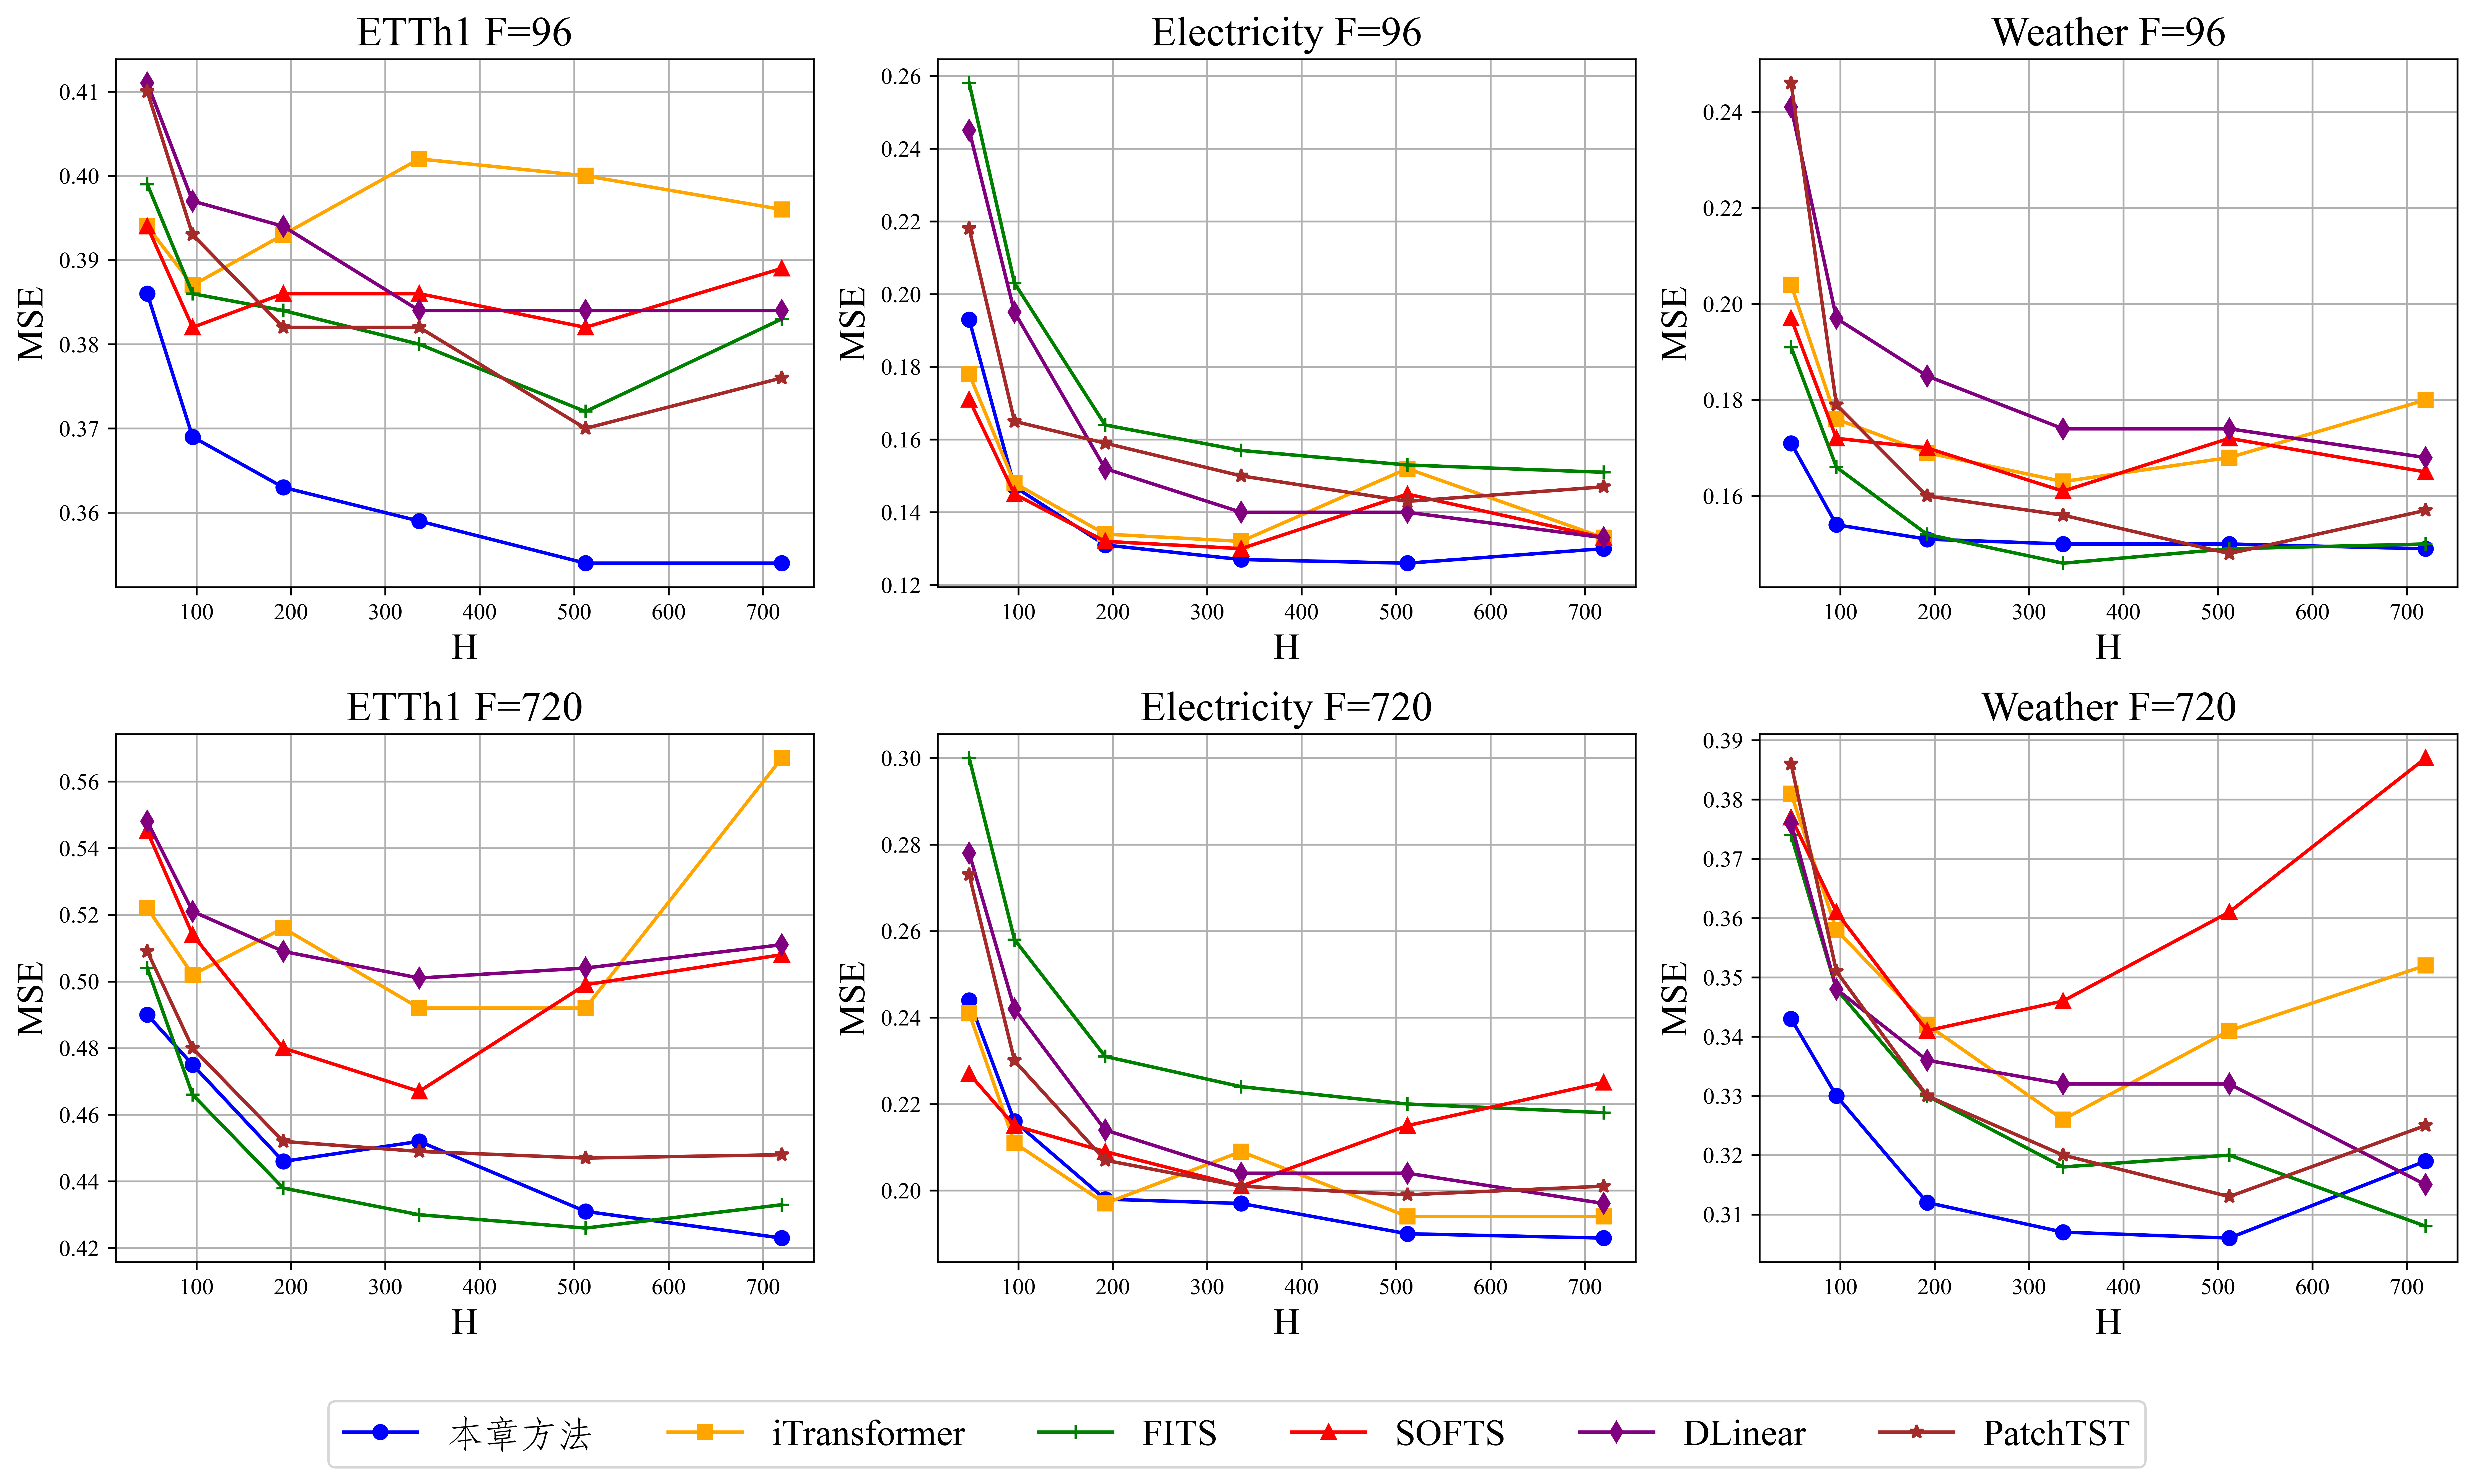
\includegraphics[width=\linewidth]{figure/ch3-lookBackVars.png}
    \caption{多元时间序列预测在不同回看窗口下的对比实验}
    \label{fig:ch3-lookBackVars}
\end{figure}

\noindent\textbf{回看窗口的影响\ \ } 历史区间长度（即回看窗口长度）决定了模型可利用的过去信息量。由于本章方法选取 Transformer 和 MLP 作为模型的基本组件，本节对比了选用这两个基本组件的基线方法进行对比，包括 iTransformer、FITS、SOFTS、DLinear 和 PatchTST。为分析回看窗口长度的影响，本节变化窗口长度 $L\in\{48,96,192,336,512,720\}$ 中，并在预测长度 $F\in\{96,720\}$ 下比较评估结果。如图~\ref{fig:ch3-lookBackVars}所示，本章方法在大多数设置下均优于选取的基线方法；随着回看窗口长度增加，模型误差总体继续下降，说明本章方法能够有效利用较长历史上下文建模长程时间依赖。

\subsection{预测结果可视化}
本节将本章方法在部分数据集上的预测结果与真值进行了可视化。回看窗口长度为 96，预测长度为 96。图~\ref{fig:ch3-predVis-Electricity}、图~\ref{fig:ch3-predVis-ETTm1} 和图~\ref{fig:ch3-predVis-traffic} 依次为 Electricity、ETTm1 和 Traffic 上的预测可视化结果。真值（Ground Truth）折线为蓝色，预测（Prediction）折线为橙色。 
\begin{figure}[t!]
    \centering
    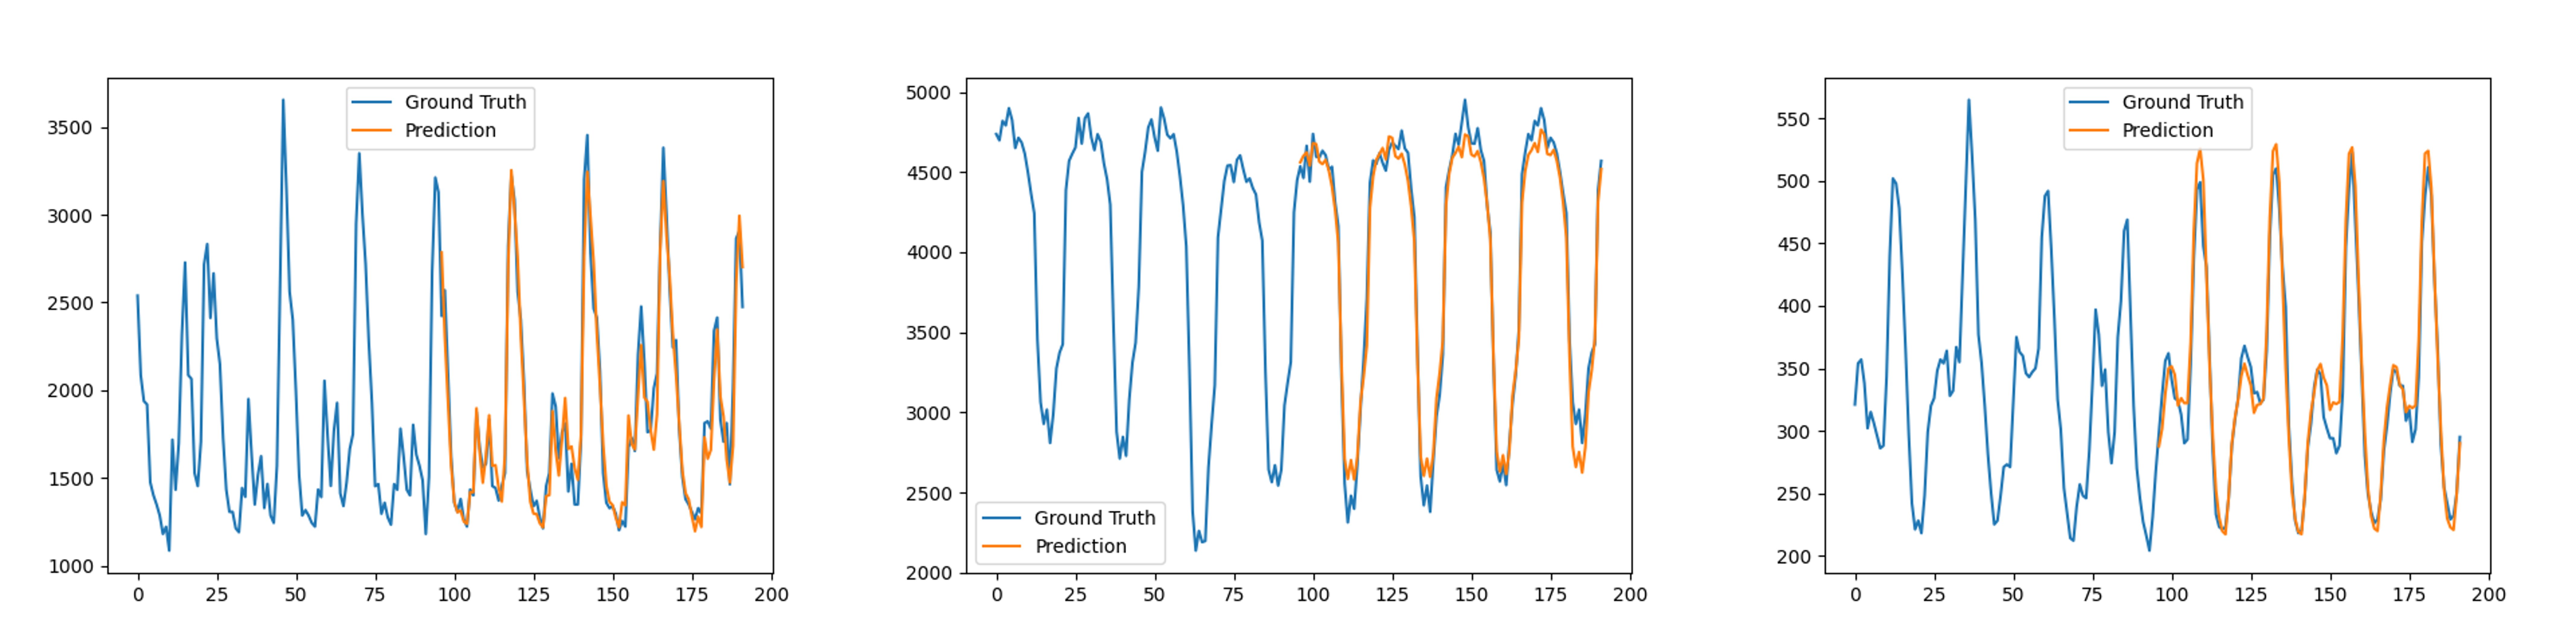
\includegraphics[width=\linewidth]{figure/ch3-predVis-ECL.png}
    \caption{多元时间序列预测方法在 Electricity 数据集上的预测结果可视化}
    \label{fig:ch3-predVis-Electricity}
\end{figure}
\begin{figure}[t!]
    \centering
    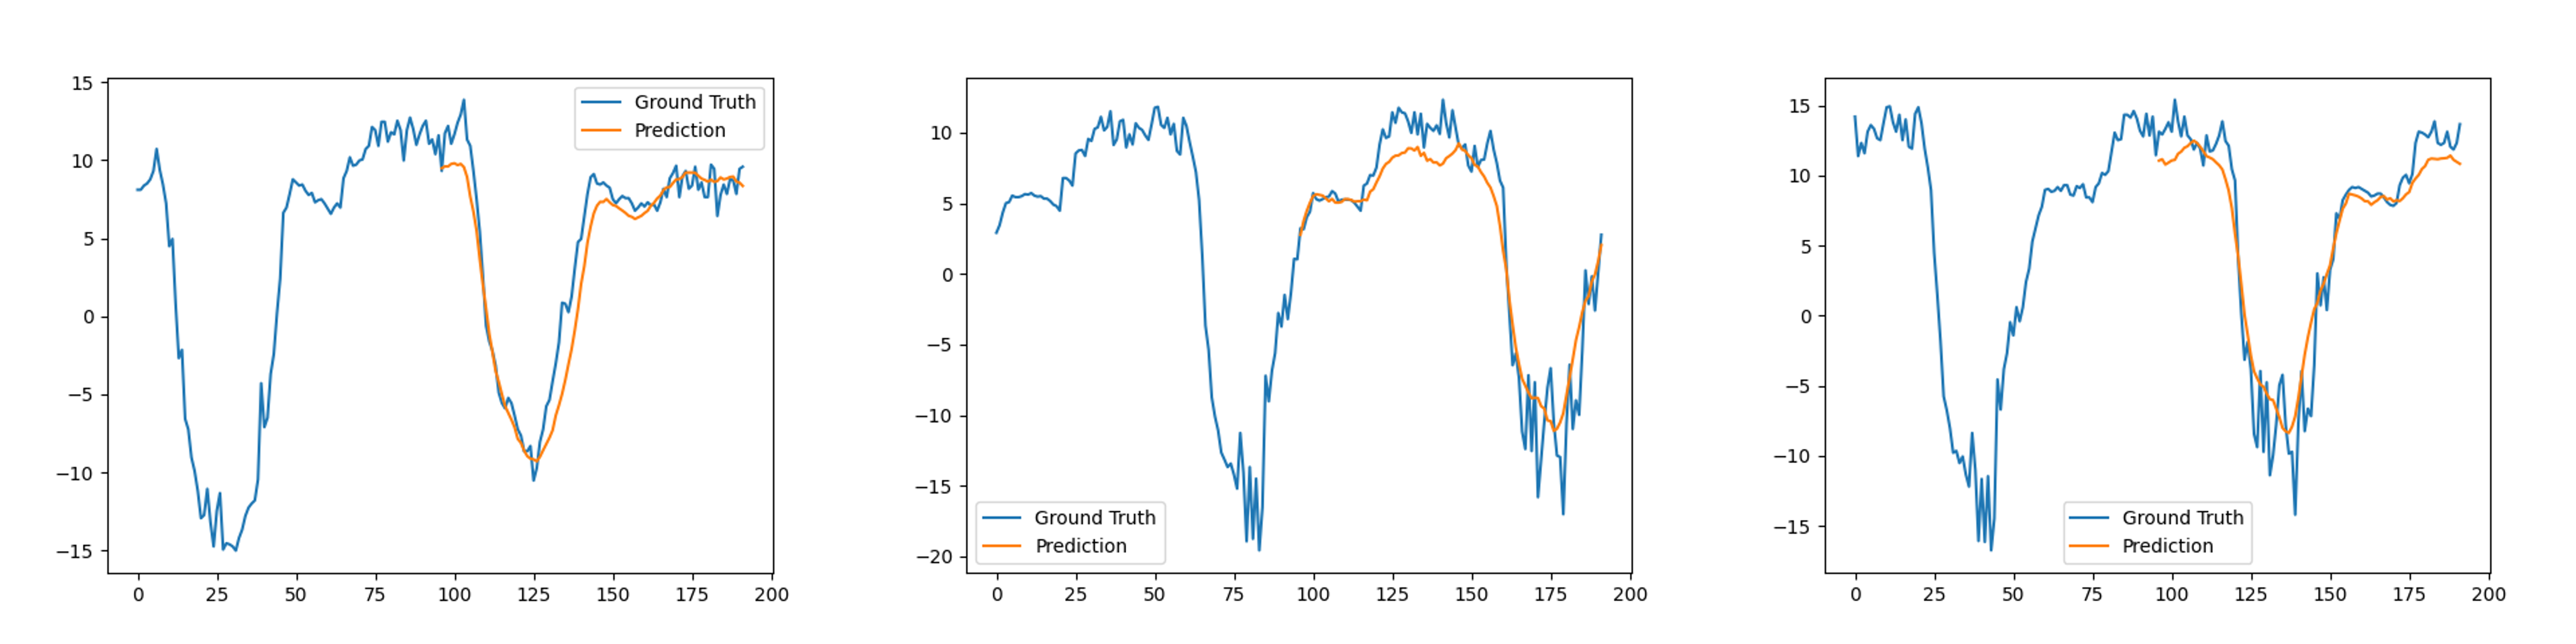
\includegraphics[width=\linewidth]{figure/ch3-predVis-ETTm1.png}
    \caption{多元时间序列预测方法在 ETTm1 数据集上的预测结果可视化}
    \label{fig:ch3-predVis-ETTm1}
\end{figure}
\begin{figure}[t!]
    \centering
    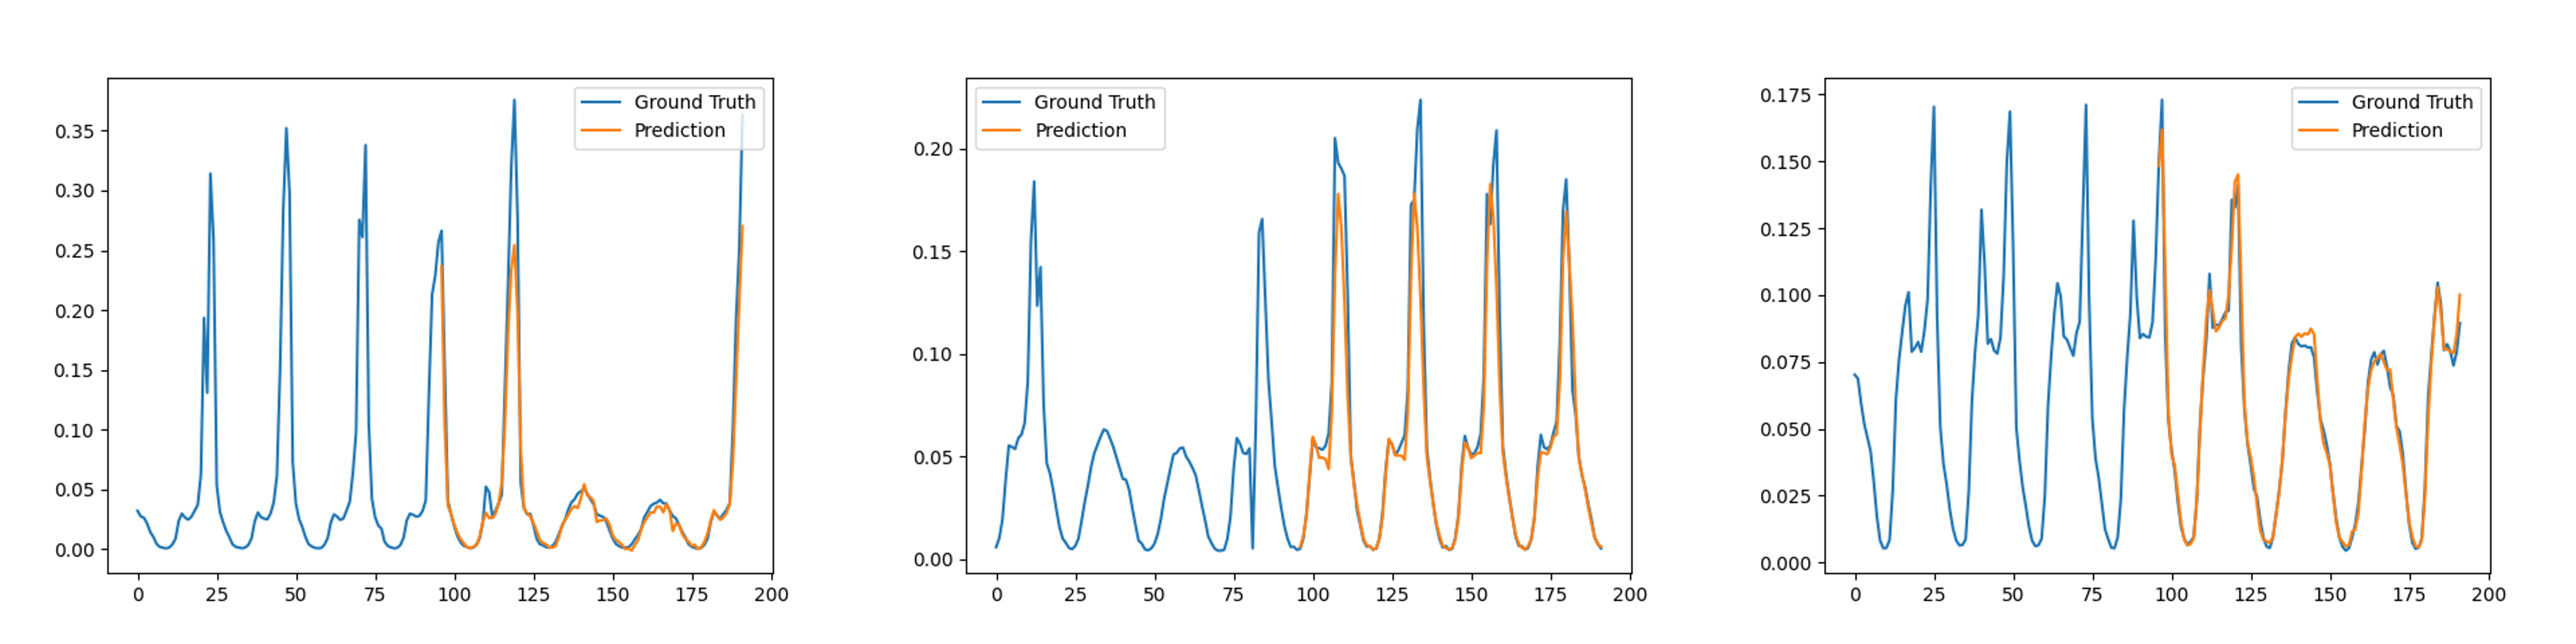
\includegraphics[width=\linewidth]{figure/ch3-predVis-Traffic.png}
    \caption{多元时间序列预测方法在 Traffic 数据集上的预测结果可视化}
    \label{fig:ch3-predVis-traffic}
\end{figure}


\section{本章小结}

本章围绕一般多元时间序列预测中时间非平稳、变量分布异质以及趋势、周期和局部波动等多尺度模式并存的问题，提出了一种融合双向时间戳依赖建模与多尺度特征提取混合专家的预测框架。与现有方法将各变量或各尺度统一建模的做法不同，本章采用通道独立路由，通过噪声门控和 Top-k 稀疏激活将不同变量动态分配给最合适的多尺度专家，从而在保留细粒度局部特征的同时增强对趋势和长程依赖的表达能力。

在特征建模方面，本章通过实例归一化缓解训练与测试阶段的分布漂移，利用可学习马氏矩阵在频域中度量变量相关性并生成稀疏相关性掩码，以减少无关变量的干扰。进一步地，时间戳双向交叉注意力模块显式建模历史区间与未来区间之间的双向依赖，并通过多尺度时间戳一致性约束将时间结构信息引入预测过程。上述设计使得模型能够同时利用数据驱动表示和时间戳先验，从多尺度、多变量和双向时序依赖三个维度提升预测能力。
在 10 个公开真实数据集上的实验表明，本章方法在 40 组预测设置中分别取得 36 组 MAE 最优和 32 组 MSE 最优，整体预测精度优于多个近期基线。消融实验验证了多尺度混合专家、频域相关性建模以及时间戳双向交叉注意力等模块的有效性；尺度数量和回看窗口的分析进一步说明了不同预测长度下模型对细粒度信息和长程趋势的依赖差异。

综上，本章方法能够有效缓解一般多元时间序列预测中的非平稳性和多尺度建模难题，并为第4章将多尺度混合专家思想扩展到具有显式空间图结构的交通预测任务提供了基础。
